\documentclass[thesis]{plai}

\usepackage{tabularx}

\usepackage{lipsum}
\usepackage{booktabs}
\usepackage{graphicx}
\usepackage{realboxes}
\usepackage{tabularx}
\usepackage{svg}
\graphicspath{{images/}}
\usepackage{rotating}
\usepackage{float}
\usepackage{fancyhdr}
\setlength{\headheight}{13.6pt}
\addtolength{\topmargin}{-1.6pt}
\usepackage{microtype}
\usepackage{color}
\definecolor{light-gray}{gray}{0.80}
\usepackage{placeins}
\usepackage[ruled,vlined,linesnumbered]{algorithm2e}
\SetKw{Continue}{continue}
\newcommand\mycommfont[1]{\footnotesize\ttfamily\textcolor{blue}{#1}}
\SetCommentSty{mycommfont}
\usepackage{tikz}
\usetikzlibrary{backgrounds,
  shapes.geometric,
  arrows,
  decorations,
  decorations.pathreplacing,
  fit,
  positioning,
  shapes.multipart,
  calc,
  trees,
  graphs,
  quotes,
  matrix }
\usepackage{adjustbox}
\definecolor{mybluei}{RGB}{124,156,205}
\definecolor{myblueii}{RGB}{73,121,193}
\definecolor{mygreen}{RGB}{202,217,126}
\usepackage{pgfplots}
\pgfdeclarelayer{background}
\pgfsetlayers{background,main}

\tikzstyle{class} = [rectangle, draw=black, fill=blue!20, text width=6em, align=center, rounded corners, minimum height=2em]
\tikzstyle{block} = [draw, rectangle, text width=2cm, text centered, minimum height=1.2cm, node distance=3cm,fill=white]
\tikzstyle{method} = [text width=6em, align=left]
\usepackage{multirow}
\newcommand{\specialcell}[2][c]{%
  \begin{tabular}[#1]{@{}l@{}}#2\end{tabular}}

\usepackage{amsthm}

\captionsetup{justification=justified}

\newfloat{lstfloat}{htbp}{lop}
\floatname{lstfloat}{Listing}
\def\lstfloatautorefname{Listing}

\usepackage{enumitem}
\usepackage{emptypage}

% ---------------------------------------------- %
\pretitle{}
\posttitle{}
\title{
    \begin{center}
        \bfseries\LARGE
        Security Testing of Web Applications with Dynamic Symbolic Execution in ExpoSE
    \end{center}
}
\preauthor{}
\postauthor{}
\author{
    \begin{center}
        \large
        Moritz Böhm
    \end{center}
}
\predate{}
\postdate{}
\date{\relax}

% ---------------------------------------------- %
\begin{document}

\pagenumbering{gobble}
\begin{center}
    \uppercase{Ludwig-Maximilians-Universität München}
\end{center}

\begin{center}
    \uppercase{Chair of Programming Languages and Artificial Intelligence}
\end{center}

\vspace*{10mm}

\begin{center}
    
\includegraphics[height=40mm]{sigillum.png}
\end{center}

\vspace*{10mm}

{\let\newpage\relax\maketitle}

\thispagestyle{empty}

\begin{center}
    \begin{large}
        \begin{Large}
            Master's Thesis \\
        \end{Large}
         in Computer Science\\
    \end{large}
\end{center}

\vspace{1cm}

\begin{center}
    \begin{large}
        Supervisor: Prof. Dr. Johannes Kinder\\
    \end{large}
\end{center}



\begin{center}
    \begin{large}
        Submission Date: \today{}\\
    \end{large}
\end{center}

\vspace{1,5cm}

\cleardoublepage{}

\thispagestyle{empty}

\vspace*{20mm}
\noindent

\makeatletter

\begin{center}
    {\textbf{Disclaimer}}
\end{center}

\begin{flushleft}
    {I confirm that this Master's Thesis is my own work and I have documented all sources and material used.}

    \makeatother

    \vspace{15mm}
    \noindent

    Munich, \today{}

    Moritz Böhm
\end{flushleft}

\cleardoublepage{}


\thispagestyle{empty}

\vspace*{20mm}

\begin{center}
    \makeatletter

    {\textbf{Acknowledgments}}

    \makeatother
\end{center}

\begin{flushleft}
    I would like to express my heartfelt gratitude to everyone who has supported me throughout the journey of this thesis.
    
    Special thanks to Professor Kinder, for introducing me to this truly fascinating topic of \textit{dynamic symbolic execution} and for enabling me to write this thesis, while providing his continuous support and help over the course of this project.
\capstartfalse

\begin{figure}[h] 
    \centering
    
\includegraphics[width=0.5\textwidth]{images/ca-plai-corn.png}
    \caption*{Special thanks to the chair of programming languages and artificial intelligence for having this cute (unofficial?) mascot}
\end{figure}
\capstarttrue

\end{flushleft}

\vspace{10mm}

\cleardoublepage{}


\chapter*{Abstract}

As web applications grow in complexity and prevalence, ensuring their security and reliability has become increasingly important.
This thesis explores the use of Dynamic Symbolic Execution (DSE) through the ExpoSE framework to automate web application testing.
Specifically, we aim to evaluate whether ExpoSE can effectively identify bugs and security vulnerabilities, with a particular focus on Cross-Site Scripting (XSS) attacks.

Our approach involves merging the client and server into a single entity, enabling DSE to generate paths based not only on the client’s state but also on server internals.
The research includes the design and implementation of an Express.js model to facilitate the testing of complex web applications.
Through systematic evaluations, we demonstrate ExpoSE’s ability to generate inputs that cover application routes and decision paths, thereby revealing both functional issues and security weaknesses.
Our findings show that ExpoSE was able to generate unique test cases and find potential vulnerabilities related to input handling and validation.


\newpage
\tableofcontents
\microtypesetup{protrusion=false}
\microtypesetup{protrusion=true}
\pagestyle{fancy}
\fancyhf{}
\fancyhead[LO]{\leftmark}
\fancyhead[RO, LE]{\thepage}
\fancyhead[RE]{\rightmark}
\renewcommand{\headrulewidth}{0pt}



% ---------------------------------------------- %
\chapter{Introduction}
\label{chapter:introduction}
Testing of web applications for possible security breaches can be done in multiple ways. Most of them require extensive explicit writing of test cases, trying to catch all edge cases and hoping they would reveal all potential threats. 

As the title of this thesis states, we used the dynamic symbolic execution (DSE) framework ExpoSE, created for and described in \citet{loring_expose_2017}


\section{Motivation}
\label{sec:motivation}

Whenever we write code, we at some point have to test it. In ideal circumstances, we test while development, as should we not, we might be in for an unpleasant surprise. Bill Gates once said:
\begin{quote}

    “… we have as many testers as we have developers. And testers spend all their time testing, and developers spend half their time testing. We're more of a testing, a quality software organization than we're a software organization.” — Bill Gates in an interview for InformationWeek \cite{bill_q_2002} 
\end{quote}
This shows, that testing is not just an often overlooked, annoying, side effect of developing software, it actually may even more important than writing the code itself.
Automating this costly testing process, therefore, is a highly coveted question, which many approaches have tried to give an answer to. 
Recently, the use of Dynamic Symbolic Execution has been adopted as an approach for automating and generating test coverage, to uncover software bugs and malicious openings, and a many frameworks for DSE testing have been developed, each with its limitations and solutions.
ExpoSE is such a framework to test software.\\
\cite{jhala_software_2009}
The severity of bugs and malicious openings depend on the kind of program and its execution circumstances: is it an offline program, just running without any outside connection, is it a program for Internet of Things (IoT), connecting hardware with the internet, like a smart thermostat, or is it a web application, holding private information, distributing data all over the world?
All of these programs can include security issues, and to find these, programs are tested extensively. 

In this thesis, we want to apply Dynamic Symbolic Execution by using ExpoSE as a framework, to test web applications. For this, we try to answer the following research questions.


\section{Research questions}
\label{sec:research-questions}


RQ1: Is it possible to reliably end-to-end fuzz test a web application using Dynamic Symbolic Execution in ExpoSE?\\
RQ2: Can it be used to reliably find security issues?

RQ2 is directly dependent on the outcome of RQ1, as should the answer to it be a definite and resound “NO”, then there is no reason in trying to answer RQ2. A test that cannot be used to test a web application in general cannot be used for security issues. If, however, it is indeed possible, then we can go ahead to see whether ExpoSE can be used for discovering security related issues and bugs. worng


% ---------------------------------------------- %
\chapter{Terminology and Theory}
\label{chapter:background}
To address the research questions posed in~\autoref{sec:research-questions}, it is imperative to first comprehend the subjects and their fundamentals. 

We start by defining  and giving an overview of the topic areas touched upon by this thesis~(\autoref{sec:defs}) and their theory,  and then explain the technologies used within the tool ExpoSE ~(\autoref{sec:defs}).

\section{Terminology and Theory}
\label{sec:defs}
To provide an overview of all the topics that will be addressed, we will begin by defining the key components of this thesis and explaining the basics to build upon in the later chapters. 

\subsection{Web Applications}
\label{sec:webapp}
A \textit{web application} has been defined as “a software application, executed by a web server, which responds to dynamic web page requests over HTTP” by the Web Application Security Consortium (WASC) ~\cite{noauthor_web_2012}. 
In simpler terms, a web application is software that runs on a server and users access it through a web browser (like Chrome or Firefox) over the internet.

Typically, the resources and scripts of web applications — such as images, text, or functionalities — are requested by the client, which is the user's computer or device, using a web browser or similar tools. This interaction follows a set of rules known as the \gls{api}, which specifies what requests can be made and how the server should respond.
The~\autoref{fig:simplified-web-app} illustrates the basic communication process between the client (the user's device), the server (where the application runs), and external services (such as another server).

Most web applications also use a database, which is a structured way of storing data, to keep information consistently available and reliable. For the purposes of this thesis, we assume that the web application has a monolithic architecture. This means that it operates as a single cohesive program on a physical computer, rather than being divided into separate parts that run on different cloud services (like AWS, or Amazon Web Services, which offers online computing power without needing dedicated hardware\footnote{https://aws.amazon.com/})
Additionally, we assume the server follows REST (Representational State Transfer) principles, which are guidelines for how web services should operate to enable smooth communication as described by \citet{roy_t_fielding_rest_2008}. 
The web server processes requests that adhere to the HTTP (Hypertext Transfer Protocol) standard, which is the foundational protocol used for transmitting data on the web (ref. ~\autoref{tab:rest_http_methods}). It can be used  with the database operations, commonly known as CRUD (Create, Read, Update, Delete) operations, as established by \citet{martin_managing_1983}, when a web application utilizes a persistent database.
This adherence ensures that the server and client can operate independently, meaning they can be developed and updated separately without affecting each other\cite{fielding_http_2022}.


\begin{figure}[ht]
    \centering
    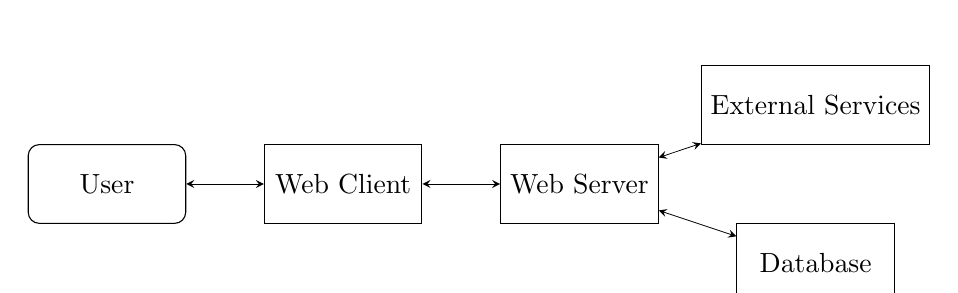
\begin{tikzpicture}[node distance=3cm]
    % Define styles for nodes and arrows
    \tikzstyle{user} = [rectangle, rounded corners, minimum width=2cm, minimum height=1cm, text centered, draw=black]
    \tikzstyle{browser} = [rectangle, minimum width=2cm, minimum height=1cm, text centered, draw=black]
    \tikzstyle{server} = [rectangle, minimum width=2cm, minimum height=1cm, text centered, draw=black]
    \tikzstyle{database} = [rectangle, minimum width=2cm, minimum height=1cm, text centered, draw=black]
    \tikzstyle{external} = [rectangle, minimum width=2cm, minimum height=1cm, text centered, draw=black]
    % Use arrows with both directions
    \tikzstyle{arrow} = [thick, <->, >=stealth]
% Arrow style for double lines

    \tikzset{doubleArrow/.style={thick, <->, >=stealth,
        line width=0.1mm, line cap=round, draw=black
    }}
    % Nodes
    \node (user) [user] {User};
    \node (browser) [browser, right of=user] {Web Client};
    \node (server) [server, right of=browser] {Web Server};
    \node (database) [database, right of=server, yshift=-1cm] {Database};
    \node (external) [external, right of=server, yshift=1cm] {External Services};
    % Arrows (connections)
    \draw  [doubleArrow](user) -- (browser);
    \draw  [doubleArrow](browser) -- (server);
    \draw  [doubleArrow](server) -- (database);
    \draw [doubleArrow] (server) -- (external);
    \end{tikzpicture}
    \caption{Structure of a simplified Web Application}
    \label{fig:simplified-web-app}

\end{figure}

\begin{table}[htb]
    \centering
    \begin{tabular}{@{}lll@{}}
        \toprule
        \textbf{HTTP Method} & \textbf{Purpose}                         & \textbf{Idempotent} \\ \midrule
        GET                   & Retrieve a resource                     & Yes                 \\
        POST                  & Create a new resource                   & No                  \\
        PUT                   & Update or create a resource             & Yes                 \\
        PATCH                 & Partially update a resource             & Yes (mostly)        \\
        HEAD                  & Retrieve headers of a resource         & Yes                 \\
        OPTIONS               & Return available HTTP methods           & Yes                 \\
        DELETE                & Remove a resource                       & Yes                 \\ \bottomrule
    \end{tabular}
    \caption{Summary of REST HTTP Methods and their idempotence \cite[chapter 9]{fielding_http_2022}}
    \label{tab:rest_http_methods}
\end{table}
\FloatBarrier
\subsection{Testing}
\label{sec:testing}

The next aspect we would like to concentrate on is the testing of a web application. First we define what "testing" means, then look into the methodology of "fuzzing" as a technique used to test. We limit this to the following two testing paradigms:
Black Box Fuzzing (\autoref{sec:black-box})and White Box Fuzzing (\autoref{sec:white-box}) .

\subsubsection{Testing}
At its essence, \textit{Testing} constitutes the systematic process of validating and verifying the functionality of a program. A sensible analogy for the concepts of validation and verification was articulated by \citet{b_w_boehm_verifying_1984}:

\begin{itemize}[label={}]
    \item \textit{Verification}: “Am I building the product right?” 
    \item \textit{Validation}: “Am I building the right product?”
\end{itemize}
Depending on the nature of the testing methodology employed, different levels of  assessment can be achieved. A unit test, which is designed to evaluate a single component or function—hence the term “unit”—primarily provides insights into the correctness of that individual function. In contrast, an end-to-end test, while potentially less precise in verifying the functionality of individual components, serves to validate the overall functionality of the entire system. 

Given that a program can accommodate a vast array of potential inputs, it may be impractical to manually identify all possible variations. Therefore, we can utilize a technique known as “fuzzing”.

\subsubsection{Fuzzing}
\label{sec:fuzzing}
\textit{Fuzzing} is an automated process that involves the generation of input data to identify potential program errors, commonly referred to as "bugs", which may arise from unhandled edge cases. These edge cases can include scenarios such as incompatible data types, excessively large entities, or the presence of unexpected characters.
The most basic idea of fuzzing is generating random input strings, which, when it was done first, already found bugs and crashes in the tested libraries \cite{miller_empirical_1990}.\\
Fuzzing can be done in different ways, and in the following we will describe the two most commonly used types: “white-box” fuzzing and “black-box” fuzzing.


\vspace{0.5cm}
\begin{tabular*}{\textwidth}{@{}c|c@{}}
    
\begin{minipage}{\dimexpr0.5\textwidth-2\tabcolsep}
\centering
    % Left Diagram - White Box Fuzzing
    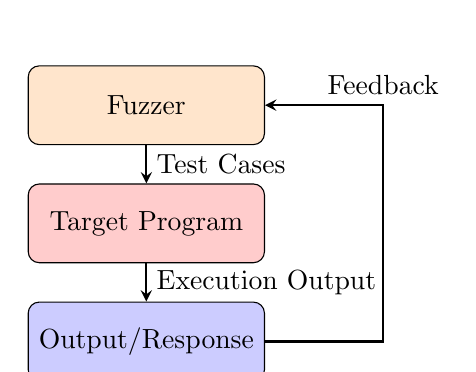
\begin{tikzpicture}[node distance=1.5cm]
                % Define styles for nodes and arrows
        \tikzstyle{box} = [rectangle, rounded corners, minimum width=3cm, minimum height=1cm, text centered, draw=black, fill=blue!20]
        \tikzstyle{fuzzer} = [rectangle, rounded corners, minimum width=3cm, minimum height=1cm, text centered, draw=black, fill=orange!20]
        \tikzstyle{target} = [rectangle, rounded corners, minimum width=3cm, minimum height=1cm, text centered, draw=black, fill=red!20]
        \tikzstyle{arrow} = [thick,->, >=stealth]
        \tikzstyle{title} = [rectangle, rounded corners, minimum width=5cm, text centered, draw=none, fill=none, font=\large\bfseries] 
    
        \node (fuzzer) [fuzzer] {Fuzzer};
        \node (target) [target, below of = fuzzer] {Target Program};
        \node (output) [box, below of = target] {Output/Response};

        % Arrows
        \draw  [arrow](fuzzer) -- (target) node[midway, right] {Test Cases};
        \draw [arrow] (target) -- (output) node[midway,right] {Execution Output};
        \draw [arrow] (output.east) --+(1.5,0) |- (fuzzer.east) node[midway, above] {Feedback};
    \end{tikzpicture}

\end{minipage}
&
\begin{minipage}{\dimexpr0.5\textwidth-2\tabcolsep}
\centering

    % Left Diagram - White Box Fuzzing
    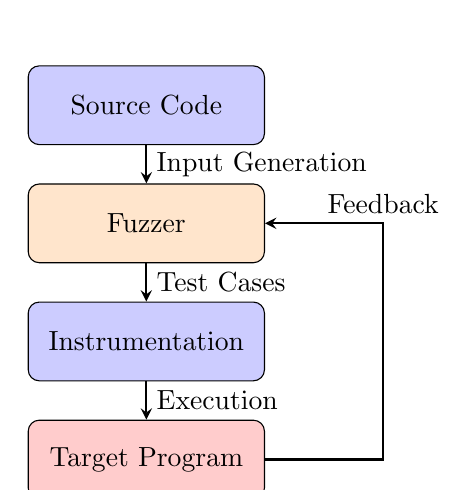
\begin{tikzpicture}[node distance=1.5cm]

        \tikzstyle{box} = [rectangle, rounded corners, minimum width=3cm, minimum height=1cm, text centered, draw=black, fill=blue!20]
        \tikzstyle{fuzzer} = [rectangle, rounded corners, minimum width=3cm, minimum height=1cm, text centered, draw=black, fill=orange!20]
        \tikzstyle{target} = [rectangle, rounded corners, minimum width=3cm, minimum height=1cm, text centered, draw=black, fill=red!20]
        \tikzstyle{arrow} = [thick,->, >=stealth]
        \tikzstyle{title} = [rectangle, rounded corners, minimum width=5cm, text centered, draw=none, fill=none, font=\large\bfseries]
        \node (source) [box] {Source Code};
        \node (fuzzer) [fuzzer, below of = source] {Fuzzer};
        \node (instr) [box, below of = fuzzer] {Instrumentation};
        \node (target) [target, below of = instr] {Target Program};

        % Arrows
        \draw  [arrow](source) -- (fuzzer) node[midway, right] {Input Generation};
        \draw  [arrow](fuzzer) -- (instr) node[midway, right] {Test Cases};
        \draw  [arrow](instr) -- (target) node[midway, right] {Execution};
        \draw  [arrow](target.east) -- +(1.5,0) |- (fuzzer.east) node[midway, above] {Feedback};

    \end{tikzpicture}
    
\end{minipage}

\\

\begin{minipage}[t]{\dimexpr0.5\textwidth-1\tabcolsep}
\captionof{figure}{Simplified black-box fuzzing process}
    \label{fig:black-box-testing}

\end{minipage}
&
\begin{minipage}[t]{\dimexpr0.5\textwidth-1 \tabcolsep}
\captionof{figure}{Simplified white-box fuzzing process}
\label{fig:white-box-testing}

\end{minipage}

\end{tabular*}

\subsubsection{Black Box Fuzzing}
\label{sec:black-box}
\textit{Black box fuzzing} (ref. \autoref{fig:black-box-testing}) is a software testing method that evaluates an application’s security and robustness by feeding it random or semi-random inputs without any knowledge of its internal workings—such as source code, data structures, or algorithms. This approach simulates an external attacker's perspective, enabling testers to discover vulnerabilities that might be exploited by malicious users in a real-world scenario.

The key characteristic of black-box fuzzing is its lack of insight into the internal design and logic of the software being tested. Instead, the focus is on the inputs and outputs of the application. Testers generate a wide variety of input data, often using automated tools or scripts, to gauge how the application responds. This can include testing edge cases, invalid inputs, or unexpected data formats to determine how robust the application is against improper use.

One of the main advantages of black-box fuzzing is its simplicity and ease of use. Since testers do not need to understand the details of the application’s code, they can quickly implement fuzzing without extensive knowledge of the underlying logic. This makes black-box fuzzing an attractive option for assessing third-party software or legacy applications where source code is not available.

Black-box fuzzing can be effective in identifying common security vulnerabilities, such as buffer overflows, input validation errors, and unexpected crashes. By observing how the application behaves with various inputs, testers can pinpoint areas of insecurity, allowing developers to focus their remedial efforts on the most critical issues.

Though black-box fuzzing offers valuable insights into application security, it does have some limitations. Specifically, the randomness of the generated inputs might not exercise all potential execution paths, leaving some vulnerabilities undiscovered. Moreover, in the absence of an understanding of the internal code structure, it may prove challenging to determine which vulnerabilities are of greater significance based on their potential impact.
 \cite{godefroid_random_2007}

\subsubsection{White Box Fuzzing}
\label{sec:white-box}
\textit{White box fuzzing} (ref. \autoref{fig:white-box-testing}) is a software testing technique that seeks to identify vulnerabilities and bugs within applications by utilizing an in-depth understanding of their internal structures and logic. Unlike traditional black-box testing methods, where testers approach the software without any knowledge of its internal workings, white-box fuzzing leverages access to the source code, algorithms, and data flows, allowing for a more targeted and effective analysis.

One of the primary benefits of white-box fuzzing is its ability to generate test inputs based on the actual paths and branches present in the code. By analysing the control flow and data structures inherent to the application, a white-box fuzzer can create specific input cases that exercise various execution paths. This targeted approach increases the likelihood of uncovering potential weaknesses, particularly in areas of the code that may be prone to errors or security vulnerabilities.

Additionally, white-box fuzzing often incorporates dynamic analysis. More on that in ~\autoref{sec:dse}. During the fuzzing process, the application is executed in a controlled environment, and its behaviour monitored in real-time. This provides valuable feedback on how the program reacts to the generated inputs, enabling the identification of unhandled cases that may lead to crashes, incorrect outputs, or security flaws.

Another critical feature of white-box fuzzing is coverage measurement. By measuring code coverage, testers can ensure that their input generation strategies are effective in exercising different paths within the software. This helps identify areas of the code that have not been adequately tested, enabling a more comprehensive examination of the program's reliability and security.

The primary objective of white-box fuzzing is to detect issues such as buffer overflows, null pointer dereferences, and other runtime errors that could compromise an application’s stability or allow for security breaches. By identifying these vulnerabilities early in the development process, organizations can address them proactively, ultimately enhancing the overall quality and security of their software.\cite{godefroid_random_2007}




\subsection{Dynamic Symbolic Execution}
\label{sec:dse}
\textit{Dynamic symbolic execution} (DSE), first presented in the seventies, is a form of white-box fuzzing, as it requires access to the source code. However, instead of requiring an actual input, it assumes that the variables are “symbolic”, meaning that they do not possess a tangible value during execution of the program. Instead, it tracks the conditions encountered during runtime, generating constraints based on the symbolic variables. 
This facilitates a comprehensive examination of multiple program pathways, thereby aiding in the identification of anomalies that may result in unforeseen behaviour or security vulnerabilities.
\cite{boyer_selectformal_1975}\cite{king_new_1975}\cite{king_symbolic_1976}\\
After exploring a particular execution path, DSE employs constraint solvers to analyse the constraints collected during execution. These solvers determine concrete inputs that can satisfy the path constraints, allowing the generation of specific test cases to trigger particular code paths during subsequent executions.

By using DSE, testers can automatically generate test cases that reliably expose bugs or vulnerabilities, such as buffer overflows or access violations. This allows for a more exhaustive testing process that can reveal flaws that traditional fuzzing techniques might overlook.

The synergy between DSE and white-box fuzzing promotes automated test generation and increases the coverage of tested paths, ultimately improving the software's reliability and security. It provides developers with concrete inputs that reproduce identified vulnerabilities, facilitating debugging and remediation.



\subsubsection{Example Dynamic Symbolic Execution}
In this subsection, we will demonstrate the concept of DSE by employing the following code snippet (\autoref{fig:example-program}). 


\vspace{0.5cm}

\begin{tabular*}{\textwidth}{@{}c|c@{}}
    
\begin{minipage}{\dimexpr0.5\textwidth-2\tabcolsep}
\centering
    % Left Diagram - White Box Fuzzing

\begin{lstlisting}[language=JavaScript, gobble=4, escapechar=@]
    function g(x, y) {
        if (x !== y){
            x += y
        }
        else {
            if (y > 8){
                y+=1
            }
        }
        x += 1
        if (x != 0 )
        { 
          if ( y != 0){
            x = y
          }
        }
    }
\end{lstlisting}
   
\end{minipage}
&
\begin{minipage}{\dimexpr0.5\textwidth-2\tabcolsep}
\centering
     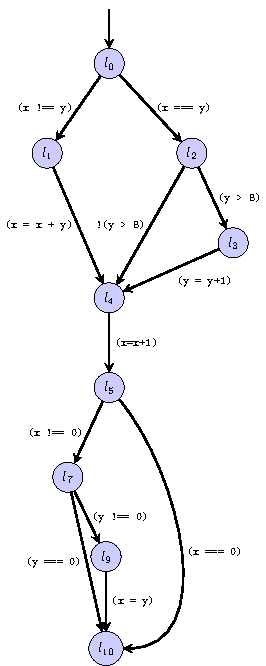
\includegraphics{../luatex/cfg/out/cfg.pdf}
\end{minipage}

\\

\begin{minipage}[t]{\dimexpr0.5\textwidth-1\tabcolsep}
 \captionof{figure}{A simple program}
\label{fig:example-program}

\end{minipage}
&
\begin{minipage}[t]{\dimexpr0.5\textwidth-1 \tabcolsep}
\captionof{figure}{CFG of \autoref{fig:example-program}}
\label{fig:example-program-graph}

\end{minipage}

\end{tabular*}
To facilitate the process, we can first depict the program as a Control Flow Graph (CFG) \autoref{fig:example-program-graph}. 
The CFG displays the conditions and transformations along its edges, with the vertices signifying the state of the program.
On entering  the program, we assume that the initial value of x=1 and y=0, just to tell the DSE Engine the types of the variables, and to give a starting point. 

\begin{center}
    We can denote this as a tuple of (pc, S(x), C(x)) 
    \begin{table}[h]
        \begin{tabular}{lll}
            where & pc & the path condition \\
             & $S(x) \rightarrow X$& the symbolic value of x, i.e. the applied transformations on the initial value\\
             & $C(x) \rightarrow 0$& the concrete value of x\\
        \end{tabular}
    \end{table}
\end{center} 
In similar fashion, we can now walk through the execution, and create a branch whenever we encounter diverging paths.
For example, right at the start, we have two possible routes the execution can take: $x == y$ and $\neg(x == y)$.
We can now construct the symbolic execution tree displayed in \autoref{fig:symbolic-execution-tree} by tracking the path conditions and transformations of the variables.

\begin{sidewaysfigure}
  \centering
  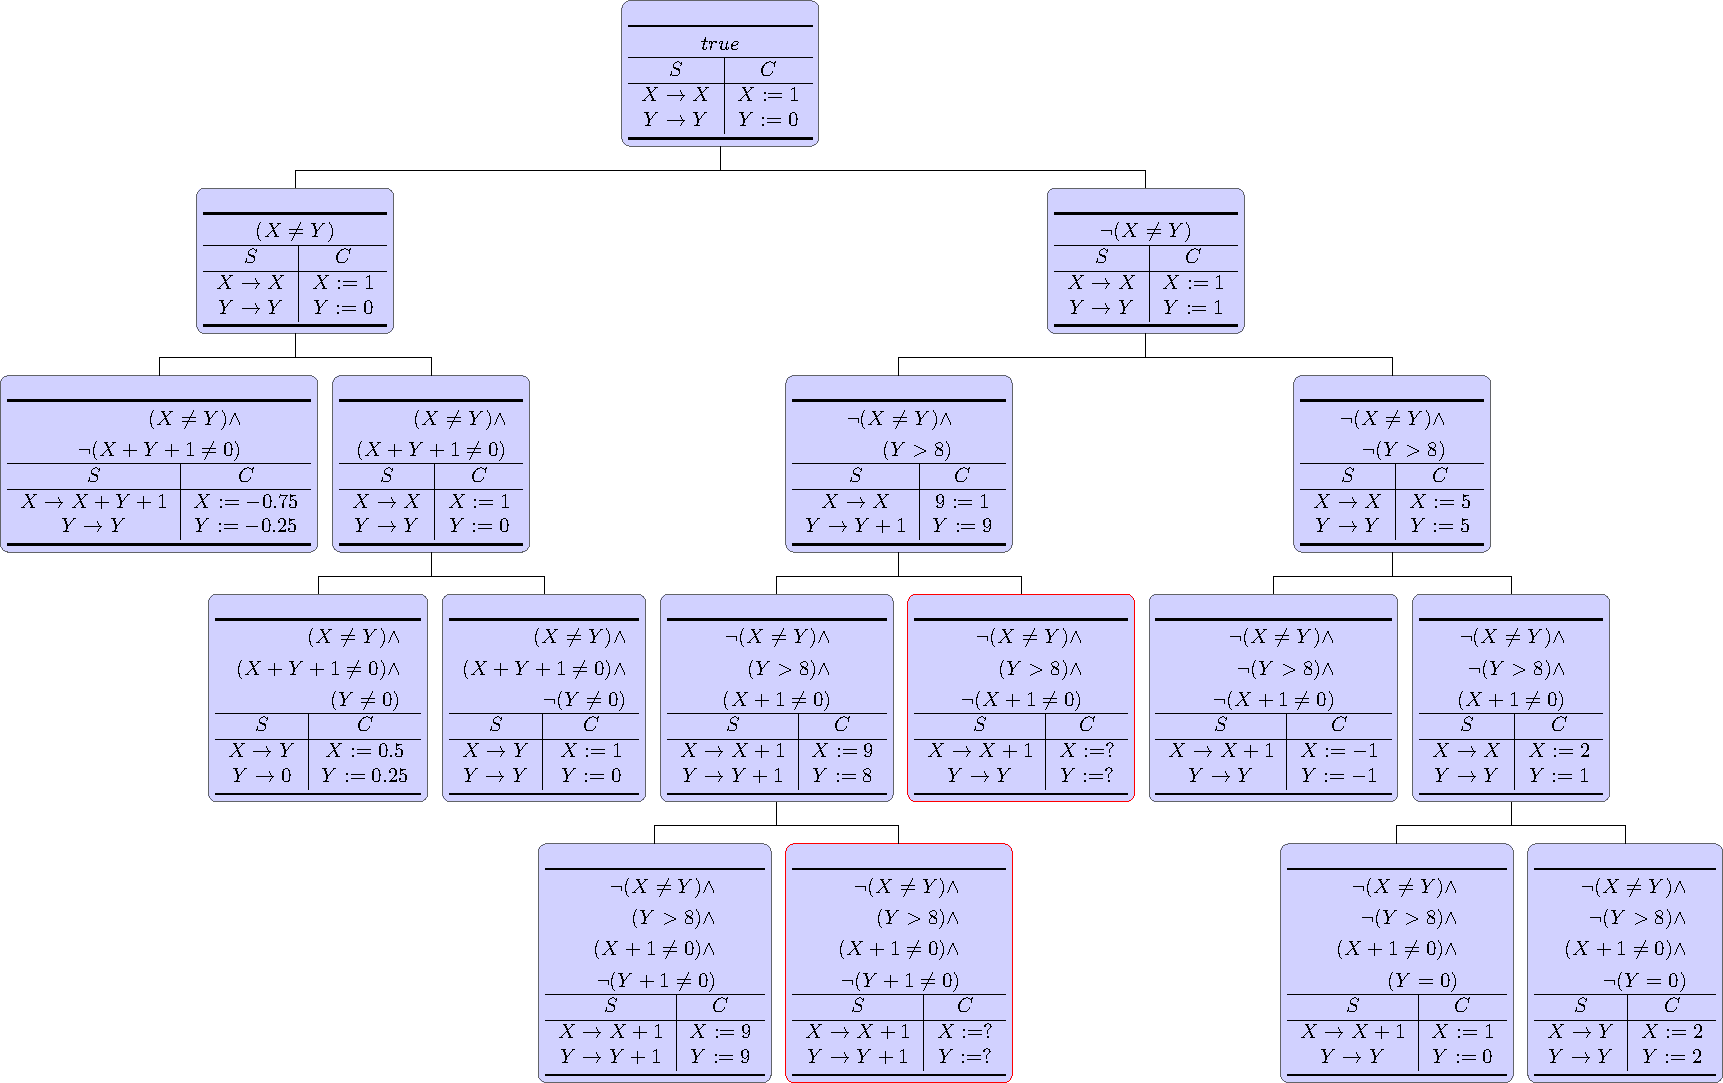
\includegraphics[width=\textwidth]{../luatex/symexe/out/symexe.pdf}    
  \caption{Symbolic execution tree of \autoref{fig:example-program} , displaying the path condition and the concolic state. Unreachable paths are highlighted in red.}
  \label{fig:symbolic-execution-tree}
\end{sidewaysfigure}




After constructing the execution tree, we can generate distinct inputs for each of the leaf nodes, checking for satisfiability.
For instance, if we want to determine which input would cover the branch in the middle of the tree, we can do so by solving the constraints  $(\neg(X \neq Y) \land (Y > 8) \land \neg( X+1==0 ) \land \neg(Y+1 \neq 0 ))$. 
Solving these constraints yields the answer of (x = 9, y = 9), which indicates that this input will satisfy the specified conditions for that branch. 
Any condition that cannot be satisfied means that the leaf node cannot be reached no matter the input. The two leafs highlighted in red in  \autoref{fig:symbolic-execution-tree} showcase this.
These constraints are usually solved by an SMT Solver, which we will briefly explain in \autoref{sec:smtsolver}.


JavaScript has a few peculiarities, as it is dynamically typed and therefore only resolved at runtime. 

\subsubsection{Limitations DSE}

As with any explorative system, DSE has limitations regarding its capabilities. 
The most significant limitation is computable paths, which have the potential to explode if the analysed program is not designed with DSE in mind, for instance, if it heavily relies on recursive calls. 
But even with DSE in mind, the paths grow exponentially with the number of conditionals in a program.  \cite{cadar_symbolic_2013}
This also occurs with symbolic addresses, as it has to account for any possible memory address a variable can occupy \cite{elkarablieh_precise_2009}.  

To address this, most DSE frameworks employ various kinds of techniques for reducing the number of paths. 
One such technique is path merging based on heuristics, where a reoccurring conditional, can be merged into one (for example in a loop)   cite statemerging kinder%TODO
\citet{cha_unleashing_2012} propose a solution for reducing the possible paths for symbolic addresses by concretizing writes and only allowing sybolic.    

It also is not suitable for boundary testing, as DSE checks for reachability, and once a path is covered, it will not move back and check for edge case in this path, possibly missing unexpected behaviour. \cite{berthier_efficient_2023}


\FloatBarrier
\subsection{SMT Solver}
\label{sec:smtsolver}

A \textit{satisfiability modulo theories }(SMT) Solver is a tool used in formal verification, automated reasoning, and various applications within computer science and engineering. The need for SMT solvers arises from the complexity of verifying whether certain logical formulas, particularly those involving rich theories such as integers, real numbers, arrays, and others, are satisfiable. Traditional propositional satisfiability (SAT) solvers face challenges with these complex theories, which is why the development of SMT solvers has become essential for enhancing automated reasoning capabilities.

SMT solvers extend the capabilities of SAT solvers by incorporating various decision procedures tailored for different theories. The process begins with the translation of a given problem into a logical formula that can be expressed in a first-order language. Initially, the SMT problem is transformed into a conjunction of logical formulas, some of which may involve theoretical constructs. Each theory, such as those pertaining to integers, arrays, or bit-vectors, possesses its own decision procedure. SMT solvers combine these procedures to handle the entire formula, typically through a technique known as "dPLL(T)," where T represents the specific theory being addressed.


When an SMT solver processes a logical formula, it checks for potential conflicts—instances in which segments of the formula cannot be simultaneously satisfied. If a conflict is detected, the solver uses conflict analysis to learn from this situation and backtrack efficiently to explore other possibilities. Throughout this process, the solver iteratively refines its search, evaluating potential assignments to variables while ensuring consistent adherence to the theoretical constraints at hand. This harmonious integration of modular theory solvers with SAT-like search techniques allows SMT solvers to effectively determine the satisfiability of complex logical formulas.\cite{barrett_satisfiability_2009}



Notable SMT solvers, such as Z3 and CVC5, have significantly impacted the field. The Z3 SMT solver, which is utilized as an SMT Solver for expoSE and was developed by Microsoft Research, has gained widespread acceptance and provides robust support for numerous theories. CVC5, developed at Stanford University, emphasizes efficiency in its decision procedures. Advances in automated reasoning have helped to establish SMT solvers as essential components in many formal verification tools, program analysis frameworks, and synthesis technologies.\cite{barrett_satisfiability_2009}


\section{Tech Stack}
\label{sec:tech}
In this section, we will delve into the inner workings of the expoSE framework, what tools it uses and their function within. 
For the following sections, we will use the following small code snippet to explain how the system works. 


\begin{figure}[h]
    \begin{lstlisting}[language=JavaScript, gobble=4]
    const S$ = require("S$");
    

    let x = S$.symbol("value"); 
    let y = S$.symbol("multiplier", 2);
    
    if (x > 0) {
        S$.assert(x*y > x, "assertion violation"); 
    }
    
   
    \end{lstlisting}
    \caption{A simple program for ExpoSE}
    \label{fig:expose-sample-program}
\end{figure}



\subsection{Jalangi}
\label{sec:jalangi}
"Jalangi2 is a framework for writing dynamic analyses for JavaScript." \cite{noauthor_samsungjalangi2_nodate}\\
Jalangi2, first presented in \citet{sen_jalangi_2013}, is used to instrument the JavaScript code that is to be analysed and provides callbacks for a program to spy onto the execution.
It enables this, by attempting to simplify every execution statement by breaking them down into atoms, which are made up of the functions listed \autoref{tab:jal-fun}, which in turn provide callbacks to hook further into the execution.
The analysing tool can implement these callbacks in order to gain insight and/or modify the return value.


To instrument the code snippet in \autoref{fig:expose-sample-program}, Jalangi2 first transforms the passed code to es6 using Babble, to ensure a consistent syntax. 
Afterward, Jalangi2 instruments the code using the JavaScript parser "acorn"\footnote{https://github.com/acornjs/acorn} to generate the AST (Abstract Syntax Tree) and then rewrites the code using Jalangi's own operatrions. This creates two files per input: 
A \{filename\}\_jalangi.js and a \{filename\}\_jalangi.json. The .js file, contains the instrumented code, similar to \autoref{fig:code-snippet}, along with the static unique instruction identifiers (iids) of each callback as a JSON object, while the .json file only contains the iids.

Although the functions exhibit variation in their parameters, they always include the iid (instruction identifier) as their primary parameter. This identifier serves as a unique reference within a JSON object, which stores an array for each statement. Each array contains critical metadata consisting of the starting line number, the column of the expression on that line, the line number where the expression concludes, and the respective column number associated with the termination of the expression.



\begin{figure}[ht]

 \lstset{basicstyle=\footnotesize}
    \begin{lstlisting}[language=JavaScript, gobble=4]
    J$.N(225, 'S$', S$, 0);             // Init S$
    J$.N(233, 'x', x, 0);               // Init x
    J$.N(241, 'y', y, 0);               // Init y
    var S$ = J$.X1(41,                  // Top level declaration
        J$.W(33, 'S$',                  // Write the result of the following:
            J$.F(25,                 // Call the function with the follwing parameter:
                J$.R(9, 'require', require, 2),// Read the value of "require"
                0)  (
                    J$.T(17, "S$", 21, false)    // Retrieve the value of the S$ object
                    ), S$, 3));
    var x = J$.X1(89,                            // Top level declaration
        J$.W(81, 'x',                            // Write the result of the following:
            J$.M(73,                                   // Call the function of:
                J$.R(49, 'S$', S$, 1),           // Read the value of the expression S$
                'symbol', 0)                     // Name of the called function
                    (J$.T(57,"value", 21, false),// Defines the value of the 
                                                 // variable as literal
            J$.T(65, 0, 22, false)),x, 3));      // Retrieve the value "0"


    \end{lstlisting}
    \caption{A shortened program snippet from \autoref{fig:expose-sample-program}, instrumented by JALANGI2, with explanation}
    \label{fig:code-snippet}
\end{figure}

As it is apparent in \autoref{fig:code-snippet}, every assignment can be traced on a granular level, enabling the analyser to know the exact state of a program, at any stage of the execution. 
If, for example, we wanted to modify, or simply log the value of the multiplier in line 24, we could do so by hooking (accessing the execution process) into the callback function provided for the function T.
This example, of course, is almost as simple as it can get. This is because JavaScript is known for having expressions that contain multiple callbacks, which in turn may or may not have callbacks themselves, colloquially called “Callback Hell” \cite{max_ogden_callback_2019}. And while an example with a callback would be a better representation of a real program, it would also mean that the instrumented code example be by a magnitude longer, rendering the example incomprehensible (not to mention, \textit{rendering} it on PDF and having it readable impossible). \\


\begin{table}[h]
\resizebox{\linewidth}{!}{%
	\begin{tabular}{l|l|l}
    {\lstinline|J$.U           |} & Unary operation                                       & {\lstinline|unaryPre|} and {\lstinline|unary|}                      \\
		{\lstinline|J\$.B           |} & Binary operation                                      & \lstinline|binaryPre| and \lstinline|binary|                    \\
		{\lstinline|J\$.C           |} & Condition                                             & \lstinline|conditional|                             \\
		{\lstinline|J\$.C1          |} & Switch key \lstinline|x in switch(x) { ... }|                    & no callback                             \\
    {\lstinline|J\$.C2          |} & case label \lstinline|C1 === C2|                                  & no own callback, uses callback of {\lstinline|J\$.C|} \\
		{\lstinline|J\$.\_          |} & Last value passed to C                                & no own callback                         \\
    {\lstinline|J\$.H           |} & hash in for-in. Wrap object \lstinline|o in for (x in o) { ... }| & {\lstinline|forinObject|}                             \\
  {\lstinline|J\$.I           |} & Ignore argument (Identity)                             & no callback                             \\
		{\lstinline|J\$.G           |} & Get a field                                              & \lstinline|getFieldPre| and \lstinline|getField|                \\
		{\lstinline|J\$.P           |} & Put a Field                                             & \lstinline|putFieldPre| and \lstinline|putField|                \\
		{\lstinline|J\$.R           |} & Read variable                                         & \lstinline|read|                                    \\
		{\lstinline|J\$.W           |} & Write variable                                        &\lstinline|write |                                  \\
		{\lstinline|J\$.N           |} & Init                                                  &\lstinline|declare|                                 \\
		{\lstinline|J\$.T           |} & object/function/regexp/array Literal                  &\lstinline|literal |                                \\
		{\lstinline|J\$.F           |} & Function call                                         &\lstinline|invokeFun|                               \\
    {\lstinline|J\$.M           |} & Method call                                           &\lstinline|invokeFun| and uses callbacks of {\lstinline|J\$.P|}   \\
		{\lstinline|J\$.A           |} & Modify and assign \lstinline|+=, -= ...|                          & uses callbacks of \lstinline|J\$.P| and \lstinline|J\$.B|       \\
		{\lstinline|J\$.Fe          |} & Function enter                                        &\lstinline| functionEnter |                          \\
		{\lstinline|J\$.Fr          |} & Function return                                       &\lstinline| functionExit  |                          \\
		{\lstinline|J\$.Se          |} & Script enter                                          &\lstinline| scriptEnter   |                          \\
		{\lstinline|J\$.Sr          |} & Script return                                         &\lstinline| scriptExit    |                          \\
		{\lstinline|J\$.Rt          |} & returned value                                        &\lstinline| \_return      |                          \\
		{\lstinline|J\$.Th          |} & thrown value                                          &\lstinline| \_throw       |                          \\
		{\lstinline|J\$.Ra          |} & Reads the return value stored by call to \lstinline|Rt()|         & no callback                             \\
		{\lstinline|J\$.Ex          |} & Uncaught exceptions                                   & no callback                             \\
		{\lstinline|J\$.L           |} & Returns the last computed value                       & no callback                             \\
		{\lstinline|J\$.X1          |} & top level expression                                  &\lstinline| endExpression               |            \\
		{\lstinline|J\$.Wi          |} & with statement                                        &\lstinline| \_with                      |            \\
		{\lstinline|J\$.endExecution|} & terminating execution                                 &\lstinline| endExecution                |            \\
		{\lstinline|J\$.S           |} & with statement                                        &\lstinline| runInstrumentedFunctionBody |            \\
	\end{tabular}}
	\caption{Jalangi2  functions, their descriptions, and their callbacks as stated in the JavaScript Documentation of the analyser}
	\label{tab:jal-fun}
\end{table}

\FloatBarrier
\subsection{Z3 SMT Solver and Z3JavaScript}
\label{sec:z3}


ExpoSE uses the Z3 SMT Solver \cite{de_moura_z3_2008} for solving the found path conditions of the analysed program. Developed by Microsoft, it has constant progress and improvements to its capabilities.

To use the SMT Solver, it offers an interface that connects a program in a higher-level language, like Python, Java, C++, or JavaScript, for which z3 offers a NPM (Node Package Manager) package since 2022. In expoSE, however, it is used in combination with the project Z3JavaScript, as, when expoSE got developed, there were no native JavaScript bindings available for Z3. 

These bindings are required to connect these higher-level languages to the core system of z3, which is implemented in C.

ExpoSE uses it to solve the path conditions generated by the first run of the symbolic execution, to yield new inputs, which in turn add new path conditions to be solved by Z3. 


Z3Javascript is a wrapper for the API of Z3, which generates the JavaScript bindings to be used in ExpoSE using ffi-napi, and builds the Z3 binary.

It then exposes functions that are used to interact with Z3, converting JavaScript types into C-types. 
Additionally, it transforms JavaScript regular expressions in order for the Z3 parser to understand them.






\newpage
\subsection{expoSE}
\label{sec:expose}
So, what exactly is ExpoSE? \\
In short, it is a DSE Framework for JavaScript, which allows almost any JavaScript code to be tested for bugs, generate tests that cover the code base to a high degree and checks for reachability of statements, by employing the aforementioned tools. \cite{loring_expose_2017}

In the following, we will demonstrate how exactly the framework operates. \\
Assume we have a small function:\\
Now, while short, there already is a lot to unpack here. Let's go over it line by line. 
\begin{itemize}
    \item Line 1: \lstinline{const S$ = require("S$")}: S\$ loads the interface library, that allows the user to interact with expoSE, declare a variable as symbolic and create assertions of conditions. More on that in the next lines.
    \item Line 3: \lstinline{let x = S$.symbol("value")}: We create a symbolic variable "x" by using the S\$ function "symbol", which allows us to define a name to track the variable with. We pass the systenm internal variable name "value" as parameter.  
    \item Line 4: \lstinline{let y = S$.symbol("multiplier", 2)}: We then create a symbolic variable “y”, internally called “multiplier”, this time, we also assign a starting seed (2), which at the same time defines the type of the variable.
    \item Line 5 to 7: then apply these variables and try to do something with them. Here, we have a simple condition ($x > 0$), which, when fulfilled, triggers the assertion \lstinline{S$.assert(x*y > x)}, which throws the exception “assertion violation”, if  the assertion is violated.
\end{itemize}
Afterwards, expoSE uses the functions exposed by the Jalangi2 backend  to access the instrumented code. For this, expoSE had to implement the callbacks of the provided backend functions. A template for these can be found in the Jalangi2 source code, with explanations for each of the functions, as part of an example analysis program\footnote{https://github.com/Samsung/jalangi2/blob/master/src/js/runtime/analysisCallbackTemplate.js}. 
It starts by registering all local variables, functions and formal parameters, in our example case the variables and constants S\$, x and y. Subsequently, it resolves the statements, loads the S\$ library and creates a concolic variable: if a concrete value is present, it uses this as starting seed. Otherwise, it will try all primitive types as the first input generation (i.e. string, array, number, object etc). The symbolic part of the concolic wrapper saves all encountered path conditions, which will be used to generate a new input which satisfies another path condition, thereby diverging from the original path, and maybe finding alternative paths.
By having the assertion \lstinline{x*y > x} we force ExpoSE to create two more paths than it normally would. Without the assertion, there are the two paths \lstinline{x>0} and \lstinline{!x>0}. But with the assertion, we added the path condition \lstinline{(x*y) > x} and its negation. This can be used to test for a certain behaviour, but requires manual modification of the program. Similar to normal conditionals, it also leads to the amount of explorable paths to explode.


% ---------------------------------------------- %
\chapter{Dynamic Symbolic Execution with ExpoSE}
\label{chapter:techstack}
In this chapter, we will delve into the inner workings of the expoSE framework, what tools it uses and their function within. 
For the following sections, we will use the following small code snippet to explain how the system works. 


\begin{lstlisting}[language=JavaScript, float, floatplacement=tbp, caption={A simple program for ExpoSE}, label={lst:expose-sample-program}]
const S$ = require("S$");


let x = S$.symbol("value"); 
let y = S$.symbol("multiplier", 2);

if (x > 0) {
    S$.assert(x*y > x, "assertion violation"); 
}


\end{lstlisting}




\section{Jalangi}
\label{sec:jalangi}
The Jalangi2 GitHub page \cite{noauthor_samsungjalangi2_nodate} states: "Jalangi2 is a framework for writing dynamic analyses for JavaScript." , and was first presented by \citet{sen_jalangi_2013}. It is used to instrument the JavaScript code that is to be analysed and provides callbacks for a program to spy onto the execution and shadow the variables.
Jalangi2 enables this, by attempting to simplify every execution statement by breaking them down into atoms, which are made up of the functions listed \autoref{tab:jal-fun}, which in turn provide callbacks to hook further into the execution.
The analysing tool can implement these callbacks in order to gain insight and/or modify the return value.


To instrument the code snippet in \autoref{lst:expose-sample-program}, Jalangi2 first transforms the passed code to es6 using Babble, to ensure a consistent syntax. 
Afterward, Jalangi2 instruments the code using the JavaScript parser "acorn"\footnote{https://github.com/acornjs/acorn} to generate the AST (Abstract Syntax Tree) and then rewrites the code using Jalangi's own operatrions. This creates two files per input: 
A \{filename\}\_jalangi.js and a \{filename\}\_jalangi.json. The .js file, contains the instrumented code, similar to \autoref{lst:code-snippet}, along with the static unique instruction identifiers (iids) of each callback as a JSON object, while the .json file only contains the iids.

Although the functions exhibit variation in their parameters, they always include the iid (instruction identifier) as their primary parameter. This identifier serves as a unique reference within a JSON object, which stores an array for each statement. Each array contains critical metadata consisting of the starting line number, the column of the expression on that line, the line number where the expression concludes, and the respective column number associated with the termination of the expression.



 \lstset{basicstyle=\footnotesize}
\begin{lstlisting}[language=JavaScript, float, floatplacement=tbp, caption={[Instrumented program snippet]Lines 1 and 4 of the program snippet \autoref{lst:expose-sample-program}, instrumented by \texttt{JALANGI2}, with explanation}, label={lst:code-snippet}]
J$.N(225, 'S$', S$, 0);             // Init S$
J$.N(233, 'x', x, 0);               // Init x
J$.N(241, 'y', y, 0);               // Init y
var S$ = J$.X1(41,                  // Top level declaration
    J$.W(33, 'S$',                  // Write the result of the following:
        J$.F(25,              // Call the function with the follwing parameter:
            J$.R(9, 'require', require, 2),// Read the value of "require"
            0)  (
                J$.T(17, "S$", 21, false)    // Retrieve the value of the S$ literal
                ), S$, 3));
var x = J$.X1(89,                            // Top level declaration
    J$.W(81, 'x',                            // Write the result of the following:
        J$.M(73,                                   // Call the function of:
            J$.R(49, 'S$', S$, 1),           // Read the value of the expression S$
            'symbol', 0)                     // Name of the called function
                (J$.T(57,"value", 21, false),// Defines the value of the 
                                             // variable as literal
        J$.T(65, 0, 22, false)),x, 3));      // Retrieve the value "0"


\end{lstlisting}

\newpage
As it is apparent from \autoref{lst:code-snippet}, every assignment can be traced on a granular level, enabling the analyser to know the exact state of a program, at any stage of the execution. If, for example, we wanted to modify, or simply log the value of the multiplier in line 24, we could do so by hooking (accessing the execution process) into the callback function provided for the function T.
This example, of course, is almost as simple as it can get. This is because JavaScript is known for having expressions that contain multiple callbacks, which in turn may or may not have callbacks themselves, colloquially called “Callback Hell” \cite{max_ogden_callback_2019}. And while an example with a callback would be a better representation of a real program, it would also mean that the instrumented code example be by a magnitude longer, rendering the example impractical (not to mention, \textit{rendering} it on PDF while ensuring its legibility). \\


\begin{table}[h]
\resizebox{\linewidth}{!}{%
	\begin{tabular}{l|l|l}
    {\lstinline|J$.U           |} & Unary operation                                       & {\lstinline|unaryPre|} and {\lstinline|unary|}                      \\
		{\lstinline|J\$.B           |} & Binary operation                                      & \lstinline|binaryPre| and \lstinline|binary|                    \\
		{\lstinline|J\$.C           |} & Condition                                             & \lstinline|conditional|                             \\
		{\lstinline|J\$.C1          |} & Switch key \lstinline|x in switch(x) { ... }|                    & no callback                             \\
    {\lstinline|J\$.C2          |} & case label \lstinline|C1 === C2|                                  & no own callback, uses callback of {\lstinline|J\$.C|} \\
		{\lstinline|J\$.\_          |} & Last value passed to C                                & no own callback                         \\
    {\lstinline|J\$.H           |} & hash in for-in. Wrap object \lstinline|o in for (x in o) { ... }| & {\lstinline|forinObject|}                             \\
  {\lstinline|J\$.I           |} & Ignore argument (Identity)                             & no callback                             \\
		{\lstinline|J\$.G           |} & Get a field                                              & \lstinline|getFieldPre| and \lstinline|getField|                \\
		{\lstinline|J\$.P           |} & Put a Field                                             & \lstinline|putFieldPre| and \lstinline|putField|                \\
		{\lstinline|J\$.R           |} & Read variable                                         & \lstinline|read|                                    \\
		{\lstinline|J\$.W           |} & Write variable                                        &\lstinline|write |                                  \\
		{\lstinline|J\$.N           |} & Init                                                  &\lstinline|declare|                                 \\
		{\lstinline|J\$.T           |} & object/function/regexp/array Literal                  &\lstinline|literal |                                \\
		{\lstinline|J\$.F           |} & Function call                                         &\lstinline|invokeFun|                               \\
    {\lstinline|J\$.M           |} & Method call                                           &\lstinline|invokeFun| and uses callbacks of {\lstinline|J\$.P|}   \\
		{\lstinline|J\$.A           |} & Modify and assign \lstinline|+=, -= ...|                          & uses callbacks of \lstinline|J\$.P| and \lstinline|J\$.B|       \\
		{\lstinline|J\$.Fe          |} & Function enter                                        &\lstinline| functionEnter |                          \\
		{\lstinline|J\$.Fr          |} & Function return                                       &\lstinline| functionExit  |                          \\
		{\lstinline|J\$.Se          |} & Script enter                                          &\lstinline| scriptEnter   |                          \\
		{\lstinline|J\$.Sr          |} & Script return                                         &\lstinline| scriptExit    |                          \\
		{\lstinline|J\$.Rt          |} & returned value                                        &\lstinline| \_return      |                          \\
		{\lstinline|J\$.Th          |} & thrown value                                          &\lstinline| \_throw       |                          \\
		{\lstinline|J\$.Ra          |} & Reads the return value stored by call to \lstinline|Rt()|         & no callback                             \\
		{\lstinline|J\$.Ex          |} & Uncaught exceptions                                   & no callback                             \\
		{\lstinline|J\$.L           |} & Returns the last computed value                       & no callback                             \\
		{\lstinline|J\$.X1          |} & top level expression                                  &\lstinline| endExpression               |            \\
		{\lstinline|J\$.Wi          |} & with statement                                        &\lstinline| \_with                      |            \\
		{\lstinline|J\$.endExecution|} & terminating execution                                 &\lstinline| endExecution                |            \\
		{\lstinline|J\$.S           |} & with statement                                        &\lstinline| runInstrumentedFunctionBody |            \\
	\end{tabular}}
	\caption[List of Jalangi2 functions]{Jalangi2  functions, their descriptions, and their callbacks as stated in the JavaScript Documentation of the analyser}
	\label{tab:jal-fun}
\end{table}

\section{SMT Solver Z3}
\label{sec:z3}

Deciding whether a logical expression is satisfiable, depending on the expression, a difficult process.
If we take the simple expression $a = b \land b= c\land c = d \land d \neq e \land e = a$, we can check the satisfiability.
From $a = b$, we deduce that $a$ and $b$ must have the same value. 
Since $b = c$, it follows that $c$ is equal to $a$ and $b$. 
By continuing this pattern, we see that $d$ must also equal $a$, $b$, and $c$. 
However, the expression $d \neq e$ states that $d$ cannot equal $e$. Since $e = a$, this places $e$ back in the equality chain, leading to a contradiction: $d$ must equal $e$ (since $e = a = b = c = d$), which conflicts with $d \neq e$.

Automating this process of checking for satisfiability is done by a \textit{Boolean Satisfiability Theories} (\gls{sat}) Solver, first introduced by  \citet{davis_computing_1960} as the Davis-Putnam algorithm, enhanced by adding backtracking, developed by \citet{davis_machine_1962}, formerly known as the Davis, Logemann and Loveland Algorithm or DLL, and nowadays usually found as Davis-Putnam-Logemann-Loveland (DPLL)-Algorithm. 

As a SAT solver is limited to boolean expressions, research for incorporating decision procedures into formal methods was done by \citet{shostak_algorithm_1978}, \citet{boyer_integrating_1988} and others, laying the foundation for modern \textit{Satisfiability Modulo Theroies}  \gls{smt} Solvers, early on called SAT-based decision procedures.
Notable improvements happened with the introduction of the tool GRASP \cite{silva_graspnew_nodate}, by adding conflict analysis to the basic backtracking algorithm, allowing non-chronological backtracking in order to solve conflicts. \citet{moskewicz_chaff_nodate} introduced a completly new solver, improving performance drastically.  





ExpoSE uses the Z3 SMT Solver \cite{de_moura_z3_2008} for solving the generated path conditions of the analysed program. Developed by Microsoft, it has constant progress and improvements to its capabilities.

To use the SMT Solver, it offers an interface that connects a program in a higher-level language, like Python, Java, C++, or JavaScript, for which z3 offers a NPM (Node Package Manager) package since 2022. In expoSE, however, it is used in combination with the project Z3JavaScript, as, when expoSE got developed, there were no native JavaScript bindings available for Z3. 

These bindings are required to connect these higher-level languages to the core system of z3, which is implemented in C.

ExpoSE uses it to solve the path conditions generated by the first run of the symbolic execution, to yield new inputs, which in turn add new path conditions to be solved by Z3. 


Z3Javascript is a wrapper for the API of Z3, which generates the JavaScript bindings to be used in ExpoSE using ffi-napi, and builds the Z3 binary.

It then exposes functions that are used to interact with Z3, converting JavaScript types into C-types. 
Additionally, it transforms JavaScript regular expressions in order for the Z3 parser to understand them.






\section{expoSE}
\label{sec:expose}
ExpoSE builds on top of the previously presented projects and technologies. Utlizing these aforementioned tools, it is a DSE Framework for JavaScript, which allows almost any JavaScript code to be tested for bugs, by generating tests that cover the code base to a high degree and checking for reachability of statements. \cite{loring_expose_2017}

In the following, we will demonstrate how exactly the framework operates, based on the small function \autoref{lst:example-program}
 
Now, while short, there already is a lot to unpack here. Let's go over it line by line. 
\begin{itemize}
    \item Line 1: \lstinline{const S$ = require("S$")}: S\$ loads the interface library, that allows the user to interact with expoSE, declare a variable as symbolic and create assertions of conditions. More on that in the next lines.
    \item Line 3: \lstinline{let x = S$.symbol("value")}: We create a symbolic variable “x” by using the S\$ function “symbol”, which allows us to define a name to track the variable with. We pass the system internal variable name “value” as a parameter.  
    \item Line 4: \lstinline{let y = S$.symbol("multiplier", 2)}: We then create a symbolic variable “y”, internally called “multiplier”, this time, we also assign a starting seed (2), which at the same time defines the type of the variable.
    \item Line 5 to 7: then apply these variables and try to do something with them. Here, we have a simple condition ($x > 0$), which, when fulfilled, triggers the assertion \lstinline{S$.assert(x*y > x)}, which throws the exception “assertion violation”, if  the assertion is violated.
\end{itemize}
Afterwards, expoSE uses the functions exposed by the Jalangi2 backend  to access the instrumented code. For this, expoSE had to implement the callbacks of the provided backend functions. A template for these can be found in the Jalangi2 source code, with explanations for each of the functions, as part of an example analysis program\footnote{https://github.com/Samsung/jalangi2/blob/master/src/js/runtime/analysisCallbackTemplate.js}. 
It starts by registering all local variables, functions and formal parameters, in our example case the variables and constants \lstinline{S$}, \lstinline{x} and \lstinline{y}. Subsequently, it resolves the statements, loads the \lstinline{S$} library and creates a concolic variable: if a concrete value is present, it uses this as starting seed. Otherwise, it will try all primitive types as the first input generation (i.e. string, array, number, object etc). The symbolic part of the concolic wrapper saves all encountered path conditions, which will be used to generate a new input which satisfies another path condition, thereby diverging from the original path, and maybe finding alternative paths.
By having the assertion \lstinline{x*y > x} we force ExpoSE to create two more paths than it normally would. Without the assertion, there are the two paths \lstinline{x>0} and \lstinline{!x>0}. But with the assertion, we added the path condition \lstinline{(x*y) > x} and its negation. This can be used to test for a certain behaviour, but requires manual modification of the program. Similar to normal conditionals, it also leads to an increasing number of explorable paths.

An example of generated path conditions of a marginally more complex system can be found in \autoref{lst:pc-appendix} containing just one path, showcasing, that these path conditions can grow to substantial size.




% ---------------------------------------------- %
\chapter{Testing Contemporary Web Applications}
\label{chapter:implementation}

This chapter provides an overview of the project in \autoref{sec:overview}, outlines the necessary modifications to the existing project to execute expoSE on the execution platform in\autoref{sec:fwd-z3}, and presents the discovered system-imposed limitations in \autoref{sec:limits}. It then presents the initial idea in \autoref{sec:init-test-plain}. Some of them were contingent upon the platform on which the program was executed. In this case, an Apple MacBook Pro with an M1 Pro chip. 

\section{Overview}
\label{sec:overview}


ExpoSE functions as depicted in \autoref{fig:expose-struc} starting from a component referred to as the distributor to orchestrate the process of symbolic execution. The distributor facilitates the transmission of inputs to the executor, which, as its designation implies, executes the program under test utilizing these inputs. The execution of the program produces a trace, which is subsequently returned to the executor. From this trace, the path condition corresponding to the input is communicated to the SMT Solver. The SMT Solver solves the constraints and then transmits the resulting model back to the executor, enabling the executor to extrapolate alternative inputs. These alternative inputs are subsequently relayed to the distributor, thereby initiating the entire process again. In scenarios where multiple alternative inputs are generated, these inputs are executed concurrently.

For our case, the program under test is not just one script, but consists of both the server and the client, but also of the express model, the request model and the response model. 



\begin{figure}
  \centering
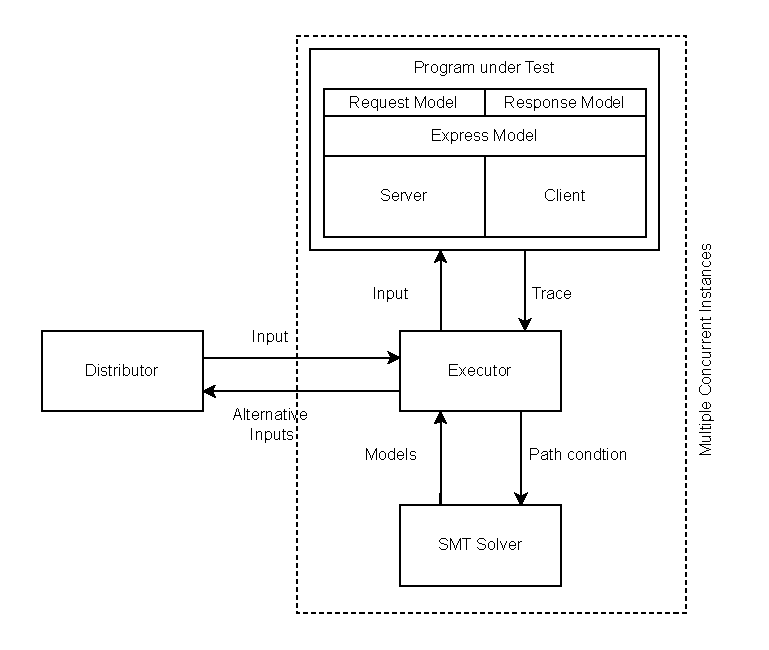
\includegraphics[width=0.7\textwidth]{exposeArchitectureDiagram.pdf}
 \caption{Express model structure, as depicted in \cite{loring_practical_2021}, modified to include the web application with the models for express, request, and response.}
     \label{fig:expose-struc}
\end{figure}


\FloatBarrier
\section{Forwarding Changes of Z3}
\label{sec:fwd-z3}
This section provides a short overview of the changes made to two of the four main parts that make up ExpoSE. Both were relatively simple in nature, but they were required to fix a z3 specific internal error, that kept occurring and caused the execution to fail.

\subsection{Changes to z3}
\label{sec:changes-z3}
As the forked repository of z3 made for expoSE was almost 5 years old, and we occasionally noticed a null pointer exception in the c++ code, we decided to pull the changes from the original repository into the fork, almost 5000 commits, in the hopes of that the null pointer exception has been fixed meanwhile. 
The forwarding went smoothly, with two exceptions. Z3 now includes the type “Char Pointer”, which had to be added to the JavaScript portion (and the Python part, as JavaScript basically copies the bindings from Python) of the binding creation.

The second exception was, that the z3 API now provided a few more callbacks, which, however, required parameters that were not implemented for JavaScript. We have chosen to eliminate these components from our fork over implementing them, as they were not utilized in expoSE and resulted in the failure of the binding generation.

\subsection{Changes to z3JavaScript}
\label{sec:changes-z3js}
With the update to z3 itself, we also had to update the z3JavaScript project, as this defined the types for the JavaScript bindings. It turned out to be a simple issue of adding two new object types (a ParserContextObj and a SimplifierObj) of the type voidp, which is a pointer to the type void.


\section{System-imposed limitations}
\label{sec:limits}
In this section, we will explain the limitations imposed on the application, what it means and how we can circumvent  some of them, while others are a hard  limit.
\subsection{JavaScript Version}
\label{sec:jsversion}
We will start off with the hardest limitation of the application, and that is the fact, that we have to stay in syntax constructs offered by the JavaScript version known as ES6 (or ECMA 2015).

This is a significant limitation, as it implies that we are unable to utilize an essential feature of contemporary JavaScript, specifically \textit{async} and \textit{await}. These two keywords refer to the asynchronous pattern that modern JavaScript employs. Without these, we will not be able to build a modern application, which is a major limitation for a server that might have to wait for resources to load or for a computation-intensive process. For these processes, we now have to rely on callbacks. 



\subsection{HTTP Protocol}
\label{sec:httpprot}
Another limitation we faced was the communication between client and server, as typically, this would happen using HTTP. However, this would mean that we would lose the symbolic state of the program, as the transfer would occur as a byte stream with all data first transformed into a string representation. 
A string, however, cannot be of symbolic type. \\
This means, we had two options:\\
Option A would require us to model the complete HTTP object, with all its bells and whistles, and then include the symbolic state of the program, all while complying with the HTTP standard. This way, we could also test HTTP, and whether the JavaScript implementation works as intended.

Option B is to bypass the transmission of data entirely, by injecting the server into the client, or vice versa, depending on the server structure (more on that later). This would mean that we would have the full symbolic state of the execution, the data would not need to be transformed, and could simply be handed over to the request and response processing on server- and client-side.


We deemed the modelling of the HTTP object out of scope. Therefore, we worked under the assumption, that HTTP works as intended and went for option B, as that meant, we could focus on the actual web application, and could test it in isolation.


\subsection{Symbolic Addresses and Objects}
\label{sec:sym-obj}
While the other limits are specific to our use case, this issue is universal, as pointers can cause a problem on most symbolic execution engines as described by \citet{cha_unleashing_2012}, \citet{coppa_rethinking_2017} and \citet{elkarablieh_precise_2009}, just to name a few. 
Reasoning about the address of a variable poses an issue, as in theory, DSE would have to assume all possible addresses. As previously mentioned in \autoref{sec:limits}, \citet{cha_unleashing_2012} proposed a symbolic address, which concretizes writes and only the read is a symbolic operation. A similar approach was also taken for ExpoSE, as it concretizes the namespace a variable can occupy, and only its value is resolved symbolically.
ExpoSE initializes a symbolic object by reserving a namespace, concretizing it.


On execution, it then tracks every property access, updating the initial object with a new symbolic variable for the accessed property. 
If we consider this expression:\\
\lstinline[language=JavaScript, gobble=4, escapechar=@]{const object = S$.symbol("object");}
This instruction initilizes the variable object as a new symbolic variable, without any indication that it is an object. 
Should ExpoSE now encounter a property access, i.e.
\lstinline[language=JavaScript, gobble=4, escapechar=@]{if(object.field === "value")},
the property \lstinline{object.field} gets initilized as a new symbolic variable
\lstinline[language=JavaScript, gobble=4, escapechar=@]{object.field = S$.symbol("field");} 
and a path condition gets added, that \lstinline{object} is, in fact, an object.\cite{loring_systematic_2021}

While this works in theory, it is incredibly costly, leading to an explosion of paths, due to the dynamically typed nature of JavaScript, thus adding one path condition per type just on encountering a property access. On black-box testing, where the program has no other option for reasoning what, using completely symbolic objects does increase coverage and helps to find bugs.
In our case, however, where we have full access to the code and where we have knowledge of all input fields, this can be avoided, by creating an object with possible properties already symbolically initialized. This can be done because all unused fields are simply ignored and not adding new path conditions. 
This means, instead of waiting for ExpoSE to find \lstinline{object.field}, we start with an object already containing the field, together with a seed indicating the type, as can be seen in \autoref{lst:sym-obj}.
\begin{minipage}{\linewidth}
    \begin{lstlisting}[language=JavaScript, gobble=4, escapechar=@]
        const object = {
            "field": S$.symbol("field", "string"),
            "numberfield"; S$.symbol("numberfield", 10),
    };
\end{lstlisting}
\captionof{lstlisting}{Concrete object together with symbolic fields initilized.}
\label{lst:sym-obj}
\end{minipage}





\subsection{External Packages}
\label{sec:externalpack}
Our last hard limit was that, even though it was possible to import and use external packages, the DSE engine would assume that any imported package was part of the code. Although technically true, it meant it would be instrumented and create execution branches. This led to a massive explosion in branches, and while it could be used to find bugs and errors in these external packages aswell, it did not offer any use for locating issues in the part of the web application we wanted to test. 
Hence, we opted out of using any external package for now.

\subsection{Dependency Issues}
\label{sec:dep-issues}
While this was not a limit per se, it proved to be an issue with executing the tool chain of expoSE in the first place. When the codebase was created in 2017, almost all personal use computers were made on an x86 platform. While ARM was already widespread in mobile devices, few personal computers were running on an ARM instruction set\footnote{We assume this to be the case, as even the \href{https://www.arm.com/-/media/global/company/investors/Arm\%20Strategic\%20Review\%20-\%202017.pdf?revision=8473a535-6f7e-4ce5-85fe-0eb6f1f75487&la=en}{investor report} in 2017 does not mention them}. Therefore, little to no effort was spent on supporting it. 
With the release of the M1 processor by Apple, this was no longer the case.
This meant that the ARM instruction set went from being rarely supported to a widely spread one.
When we started working on this thesis, we noticed the lack of support. The project required Node version 14, and the package ffi-napi\footnote{https://www.npmjs.com/package/ffi-napi}, that provided the ability to create C bindings, which were used in z3, required Node 16 or higher.
Upgrading the node version initially, would in turn create an error in ffi-napi for the ARM-based M processors~\footnote{As reported in issue https://github.com/node-ffi-napi/node-ffi-napi/issues/248}.\\
While working on this project, the issue got resolved.



\section{Initial Test Plain JS Application}
\label{sec:init-test-plain}
After addressing all the fundamental issues, we began by creating a small server in plain JavaScript to explore whether it is possible to generate requests, process them, and return the correct response for the request. For example, a GET request with the URL '/test' is handled by a GET route registered as '/test', and not incorrectly by the POST route. 

\subsection{Idea}

The objective was to construct a plain JavaScript server by utilizing the http package's method “createServer” and subsequently eliminating all components that depend on http, thus skipping the actual server-client connection.
We had two goals for this: 
\begin{itemize}
    \item  We created a server that had both static and variable routes, notably one route that consisted only of a regular expression, to test whether all routes could be found by the symbolic variable for the path alone.
    \item  We also implemented a short test for injecting code into the response, by asserting that the client cannot send any script tag \lstinline{<script><\script>} in the request data, while asserting that it has to be a valid email. Which in turn meant, expoSE has to try to violate the assertion, by creating inputs, that contain a script tag and are no valid emails. 
\end{itemize}
For the client side we created a bare-bones client, that was generating the symbolic request, and passed it over to the server by calling the onRequest method of the server, which gets called whenever a request is sent, thereby bypassing HTTP. 

\subsection{Evaluation}
This, albeit small test application, showed us, by fulfilling both of our expected outcomes, that it indeed is possible to test a server with expoSE. Finding all the request routes within the server was straightforward, with a minor drawback: the regular expression route was not functional in a switch-case construct due to its use as a literal and not as a regular expression to match a string. 
The second objective was only moderately successful, as, despite demonstrating theoretically that the generation of a string containing a script tag works, it often exceeded the timeout limit, with a few exceptions in a test of 50 runs, where a matching string was immediately generated.

Despite this, we deemed the initial test application a success, as it strongly suggested that it is possible to test a server, explore all possibly routes and locate issues in the validation, data processing and usage of this data. Hence, we moved on from plain JavaScript to the usage of a framework, in our case, Express.js.


% ---------------------------------------------- %
\chapter{Express Model}
\label{chapter:express}
This chapter presents a model implementation of the JavaScript server framework Express in \autoref{sec:overview} that enables testing a web application built with Express in its entirety through ExpoSE. It highlights the possibility of developing a model for a framework to test a web application without needing to test the framework itself. For the model to be effective, it must accurately represent the framework's core functionalities, including routing, as described in \autoref{sec:routing}, and request processing, described in \autoref{sec:req-handling}. By using the model as an abstraction layer, there is no need to create a symbolic representation of an HTTP request. We also highlight the importance of parameterized routing in our model in \autoref{sec:param-route}.

\section{General Structure}

This section provides an explanation of the general structure of the model and the internal logic of the routing, request handling, with a particular focus on the parametrized routing logic. An overview of the general structure for ExpoSE can be seen in \autoref{sec:overview}.

The model is split in two parts, as can be seen in \autoref{fig:express-struc}. On the left side, we have the request processor creation — a stack which contains all the routes and middleware for the server. For consistency purposes with Express, we will call it a stack, but for simplicity of the model, we designed it as a queue, which gets processed first in first out (right to left in the diagram). This is opposed to being reliant on calling the method “next” — in the model it returns straightaway. 
This stack can take as many layers as required, and has no minimum of middleware layers and routes, leading to every request generating an error response. 



On the right side, we have the request handling and the entry point for any request. 
Express creates an HTTP server when the method \textit{listen} is called, and opens the entry point of the Express server. As the request is handled internally of Express, we could not inject the server controller into a client, therefore requiring us to rethink the approach. This led us to switch from injecting the server code into the client, to injecting the client into the server. 

With this approach, all that was required was to slightly modify the “listen” method and pass the request directly to it as a parameter. As a result, we had a functioning server that could receive requests. Although the “listen” method usually does not return anything, we required a way for the client to receive the response again, which is why the modelled “listen” method returns the response.
To generate the request, the server was required to instantiate the client. This resolved the issue of bypassing HTTP in Express. 
Next we move on to the explanation of the model itself and how it internally handles the request and routing.

\begin{figure}[t]
        % Left Diagram - White Box Fuzzing
    \centering
    \begin{adjustbox}{width=\textwidth}
    \begin{tikzpicture}[stack/.style={rectangle split, rectangle split parts=#1,rectangle split horizontal,draw, anchor=center}]

        \tikzstyle{block} = [draw, rectangle, text width=2cm, text centered, minimum height=1.2cm, node distance=3cm,fill=white]

        \tikzstyle{target} = [rectangle, rounded corners, minimum width=3cm, minimum height=1cm, text centered, draw=black, fill=red!20]
        \tikzstyle{box} = [rectangle, rounded corners, minimum width=3cm, minimum height=1cm, text centered, draw=black, fill=blue!20]
        \tikzstyle{container} = [rectangle, minimum width=3cm, minimum height=1cm, text centered, draw=black, fill=gray!20]
        \tikzstyle{title} = [rectangle, rounded corners, minimum width=5cm, text centered, draw=none, fill=none, font=\large\bfseries]
        \tikzstyle{arrow} = [thick, ->, >=stealth]
        \tikzset{doubleArrow/.style={thick, <->, >=stealth,
        line width=0.1mm, line cap=round, draw=black
    }}

        \node (listen) [box, yshift = 1cm] {\lstinline{listen}};

        \begin{scope}
          \node (use) [box, left = of listen, xshift = -3cm ]{\lstinline{use}};      
          \node (middleware) [box, below = of use, xshift = 2cm] {\lstinline{middlware}};
          \node (router) [box, left = of middleware] {\lstinline{router}};
        
        
        \node (stack)[stack=5, below = of middleware, xshift = -2cm,fill=orange!20]  {
            \nodepart{one}\lstinline{route} 
            \nodepart{two} \lstinline{route}
            \nodepart{three} \lstinline{route}
            \nodepart{four} \lstinline{middleware}
            \nodepart{five}  \lstinline{middleware}
            };
          \node (handle) [box, below = of listen] {\lstinline{handleStack}};
        %
          %\draw  [arrow](use) -- (listen) node[midway, above] {entry point};
        \draw  [arrow](use) -- (middleware) node[midway, right] {use Middleware};
        \draw  [arrow](use) -- (router) node[midway, left] {use Router};
        \draw  [arrow](router) -- (stack) node[midway, left] {place on stack};
        \draw  [arrow](middleware) -- (stack) node[midway, right] {place on stack};
        \draw  [doubleArrow](handle) -- (stack.north east) node[midway, right] {generate response};
        \draw  [doubleArrow](listen) -- (handle) node[midway, right] {process request};
        
        \draw[->, thick] (stack.south east)  -- ++ (0,-0.2) -- ++(-6.4, 0)   node[midway, below] {process request};

        \draw[lmugreen!80,thick,dotted] ($(listen.north west)+(-1.2,0.9)$)  rectangle ($(stack.south east)+(6.4,-0.9)$)node[box]{request handling};
        \draw[blue!98,thick,dotted] ($(use.north west)+(-2.4,0.9)$)  rectangle ($(stack.south east)+(0.5,-0.9)$)node[box]{stack creation};        

        \end{scope}
    

    \end{tikzpicture}
    \end{adjustbox}
    \caption{The express model structure.}
    \label{fig:express-struc}
\end{figure}


\section{Routing} 
\label{sec:routing}
Being the most vital component of any server, routing must be implemented accordingly to enable all the features offered by Express, while removing those intended for handling a genuine HTTP request. This implies that the model must mimic how Express builds its internal routing stack, handles any incoming request, and manipulates the response. 
There are two methods to add a route to the server:

The first method is to add it directly to the server via one of the 5 HTTP methods (listed in \autoref{tab:rest_http_methods}), which takes the provided URL pattern, the callback function and its HTTP Method and places it on the stack.

The second method is to create a separate router object, which also offers the available HTTP methods. The idea for this is, that it is possible to extract the routing logic from the core server. This provides the possibility to restrict access to, add, and remove entire sections from the server without the necessity to modify the base server.

This router object then is attached in the server to a base route, most commonly in a simple server under the base route “/”, finalizing the route by which the resource can be reached. All routes are subsequently added into an array within the router. The array creation is then handled by a “use” function (\autoref{fig:express-struc} top left), which takes as many parameters as needed, which results in the following 3 cases:
\begin{itemize}
    \item  no string is provided - the callbacks are attached to the base path of "/"
     \item  the first element is of type string - this leads to adding all callbacks to the path of the first element
    \item  the second argument is of type “Router” — this leads to adding all routes added to the router to be pushed onto the stack
\end{itemize}
If, for instance, when we add the following four elements to the array:    
\begin{itemize}
    \item \lstinline[language=JavaScript]{app.use("preprocessRequest", callback(req,res,next))} - add a middleware layer, which will pre-process a request
    \item \lstinline[language=JavaScript]{app.get('/getWithId/:id', callback(req, res, next))} - add a GET request without router
    \item \lstinline[language=JavaScript]{router.post('/post', callback(req, res, next))} - add a POST request via a router
    \item \lstinline[language=JavaScript]{app.use("modify response", callback(req, res, next))} - add a middleware layer, which will post-process a request
\end{itemize}
This yields an array of object containing the routes and middleware layers as depicted in \autoref{lst:stack-example}.
\begin{lstlisting}[language=JavaScript, label={lst:stack-example}, float=top,
	caption={The routing stack created by the express model.}]
[
    {
        path: '/',
        handle: [Function (anonymous)],
        method: 'use',
        route: null
    },
    {
        route: {
            path: '/getWithId/:id',
            methods: [GET],
            parameters: [GET: "id"],
            GET: [Function (anonymous)]
        },
        path: /^\/getWithId\/(\d{1,4})$/,
        handle: [Function (anonymous)],
        method: 'GET'
    },
    {
        route: {
            path: '/post',
            methods: [POST],
            parameters: {},
            POST: [Function (anonymous)]
        },
        path: /^\/post/,
        handle: [Function (anonymous)],
        method: 'POST'
    },
    {
        path: '/',
        handle: [Function (anonymous)],
        method: 'use',
        route: null
    }
]
\end{lstlisting}

The stack comprises not only of routes, but also all middleware that is associated with the server, responsible for pre- and post-processing any request. Common middleware would include, for instance, an authorizer middleware, which verifies whether the client has the authorization to request the resource, or a logger for writing events to an output with the purpose of tracing requests.
Express requires that the middleware layers that preprocess the request and response be placed first, and any post-processing middleware be placed last, as the processing of the stack is queue-like, first in first out (hence our hesitation to call it a stack). This is done by ordering the execution statements in the same order.
Each layer object consists of four fields: method, path, handle and route.\\
The field \textit{method} has two distinct usecases. The first is signifying that it is a middleware layer, by containing the keyword "use", which will be executed no matter the request.
The second usecase is to hold the information which HTTP method it expects. \\
The field \textit{path} holds the URL pattern, which a request has to match in order for it to be processed. Should a request match the path, a flag is set that it has been matched and the model will no longer try to find a matching route. A middleware layer will always be attached to the basepath "/"\\
The field \textit{handle} contains the callback function.\\
The field \textit{route} contains all information regarding the routing layer, such as path parameters, the callback function and the HTTP methods. A middleware layer does not have such information, thus it is always null.

\section{Request Handling}
\label{sec:req-handling}
The approach to request handling is designed to replicate the method employed by Express for handling requests. This is accomplished by iterating over the stack, utilizing all middleware layers to preprocess the request, and subsequently attempting to match the request URL with an existing route pattern within the stack. When a match is identified, the request is processed, and a response is generated by invoking the callback function stored in the handle field of the corresponding routing object.

To ensure the correct functioning of this process, it is imperative that the base route, “/” is added last in the stack. This arrangement allows for the appropriate handling of all preceding routes. Additionally, a flag is established to indicate that the request has been processed, thereby preventing any possibility of matching a second route inadvertently. Finally, any post-processing middleware is applied prior to the transmission of the response to the client.

\begin{algorithm}[t]
\caption{Process incoming request - HandleStack}
\KwData{$this.stack$}
\KwIn{$request$, $response$}
\If{$request.url$ is undefined \textbf{or} $request.method$ is not in $HttpMethods$}{
\tcp{Return error response}
response $\gets$ error\;
\Return response\;
}
foundCorrectPath $\gets$ false\;
\For{each $middleWare$ in $this.stack$}{
    \tcp{Execute pre- or postprocessing layer}
    \If{$middleWare.method$ is ``use''}{
        Call $middleWare.handle(request, response)$\;
        \Continue
    }
    \Else {
        \tcp{Found a route that matches the request}
        \If{$middleWare.method$ equals $request.method$ \textbf{and} foundCorrectPath is false}{
            \If{$middleWare.path$ matches $request.url$}{
                foundCorrectPath $\gets$ true\;
                Call \texttt{processMiddleWare(middleWare, request, response)}\; 
                \Continue
            }
            \Else{
                \Continue
        }
        }
        
    }
}
\If{foundCorrectPath is false}{
response $\gets$ error\;
\Return response\;
}
\Return response\;
\end{algorithm}


\section{Parametrized Routing}
\label{sec:param-route}

It is noteworthy that the extraction of parameters sent as route variables must remain symbolic. For instance, when the route is defined as seen in \autoref{fig:param-route}, the request path might look like \lstinline[language=JavaScript]{var path = S$.symbol("path", "/user/1");}.


\begin{lstlisting}[language=JavaScript,label={fig:param-route},caption={A parameterized route.}, float]
router.get('/user/:id', callback) 
\end{lstlisting}

\begin{lstlisting}[language=JavaScript, gobble=4,caption={Parameters extracted from the request path.},label={fig:param-extracted}, float]
req.parameters =  {
    id: ConcolicValue {
        concrete: '1',
        symbolic: Expr {context: [Context], ast: [Object], _fields: [], checks: []},
    }
}
\end{lstlisting}
As illustrated in the second layer from the top in \autoref{fig:stack-example}, it  introduces a “parameters” field, which contains an object representing the parameter variable name, specifically “id”. During the processing of a request, this parameter is extracted from the path, resulting in an object that is subsequently attached to the request, as depicted in \autoref{fig:param-extracted}.
The significance of this process is that the parameter remains a concolic variable, thereby preserving its symbolic characteristics. Therefore, it becomes possible to generate additional path conditions as the request parameters interact with conditionals, facilitating the creation of corresponding inputs.

\begin{algorithm}[t]
\caption{ProcessMiddleWare}
\KwIn{$middleWare$, $request$, $response$}
\tcp{Associate path paramters with their corresponding field names}
values $\gets$ match of $request.url$ with $middleWare.path$ excluding first element\;
\For{each (key, index) in $middleWare.route.params[middleWare.method]$}{
    $request.params[key] \gets values[index]$\;
}
\tcp{Invoke callback stored in middleWare}
Call $middleWare.handle(request, response)$\;
\end{algorithm}


\section{Necessary Modifications} 
\label{sec:nec-mods}

Since the model is located in ExpoSE right now, all it requires is a slight modification to the imports and how express is called, i.e. the import requires the relative path, and cannot be imported via the node package manager (NPM). 
The usage is also slightly different, as the express model instance needs to be initiated after importing, while Express itself is initiated when it is imported. 
Other than that, it can be used just like Express, as the basic methods are implemented.


\section{Testing} 
\label{sec:app-testing}
To carry out the end-to-end testing of a web application, we require a client that has the following properties:\\ 
First, it must utilize the S\$ library, which serves as the interface to ExpoSE, as explained in \autoref{sec:expose}. 
Subsequently, all variables within the request should be substituted with symbolic inputs. 
In instances where the server expects a complex data structure in the body of the request,
it is advisable to send an object encapsulating all fields that the server can process across all routes.
This recommendation stems from the challenges associated with symbolic objects, as discussed in \autoref{sec:sym-obj}. 
This approach allows for the generalization of a single test without necessitating multiple executions to cover all required fields,
as any fields not utilized by the specific route are ignored. 
A client such as  \autoref{lst:client-example} could be used to generate the requests.

\begin{lstlisting}[language=JavaScript, float, caption={[Example Client]An Example Client for symbolic requests}, label={lst:client-example}]
const S$ = require("S$");
const { Request } = require("../request");
const { Response } = require("../response");
import HttpMethods from "../express_model/http_methods.enum";


generateRequest (){
    const req  = new Request(
        S$.symbol("path", "/"),
        HttpMethods[S$.symbol("method", 0)],
        {
            "field": S$.symbol("data", "")
        }
    )
    return req;
}
\end{lstlisting}

As explained in \autoref{sec:init-test-plain}, we use our mock implementation for the request and response objects. In the \lstinline[language=JavaScript]{generateRequest} function, we build the symbolic request, which has at least 2 parameters, a URL, and an HTTP method. For the URL parameter, we create a symbolic variable \lstinline[language=JavaScript]{path}, with the seed input \lstinline[language=JavaScript]{"/"}, eliminating all variable types but string. 
We then pass an array containing all http methods, accessing the element via the symbolic index variable \lstinline[language=JavaScript]{method}, with a starting seed like before, to indicate it being an integer.
Additionally, we create an object containing a symbolic field, which corresponds to an expected field in the server. As previously mentioned, we do not recommend using a symbolic object.


Testing a web application using the model is a straightforward process.
By injecting the client into the server code and invoking the \textsc{listen}
function  that typically converts an input into an HTTP request, \lstinline[language=JavaScript]{let response = server.listen(8080,callback, << SYMBOLIC } \par\noindent\lstinline[language=JavaScript]{CLIENT REQUEST >> );}, it becomes feasible to generate inputs that test all routes, incorporating various parameters and bodies.


Once the client is either modified or created to produce a symbolic request, 
a singular execution of ExpoSE should suffice to generate diverse requests that effectively cover all possible paths of a request and trigger all potential unique responses, as long as it is a distinct and reachable path.  

There is also the option to unit test the server functions without a client or the express model. However, this does not leverage the power of symbolic execution, as it only generates inputs for a function, instead of the whole system, requiring, albeit few, manual generation of tests for each function.



% ---------------------------------------------- %
\chapter{Evaluation}
\label{chapter:evaluation}
In this chapter we will describe our methodology and approach in regard to testing the underlying model (as explained in \autoref{chapter:express})and evaluating our results, finally answering the research questions posed in \autoref{sec:research-questions} 40 pages ago.
\section{Methodology} 



\section{Results}
Foremost: Testing a web application using DSE already provides the benefit of finding unhandled errors, such as missing undefined checks, empty request bodies etc.



\section{Discussion}

% ---------------------------------------------- 
\chapter{Discussion}
\label{chapter:discussion}
In this chapter, we present our findings in \autoref{sec:findings}, discuss discovered limitations in \autoref{sec:limitations} and provide our thoughts on further research and work in \autoref{sec:ft-research}.

\section{Findings}
\label{sec:findings}
Our findings are based on the presented results in \autoref{sec:results}, and the experiences we gained during the research for this thesis.

\subsection{Reliability of End-to-End Testing}
Using ExpoSE combined with Dynamic Symbolic Execution provided clear insights into the testing capabilities for web applications. As presented in \autoref{sec:results}, our efforts resulted in the moderately successful testing of two web applications using our Express model. We were able to generate inputs that thoroughly covered almost all defined routes and effectively addressed decisions that rely on correct path parameters. By automatically generating diverse inputs, ExpoSE explored the application's functionality, helping us identify unique paths in the application. Unfortunately, we encountered one path that did not get explored, which might be an indication that the reliability is questionable at best. This, however, is because ExpoSE does require unique path conditions, which the route in question did not create.
Thus, we think that ExpoSE can be utilized for testing web applications. Its capabilities in generating inputs that traverse different routes and decision points substantiate its effectiveness in revealing hidden issues that may arise in complex application structures. 


\subsection{Identification of Security Vulnerabilities}
The framework provides valuable insights into allowed inputs by generating test cases that include potential attack patterns within strings. If the malicious string was already stored in the database, ExpoSE was unable to pinpoint the malicious content.

Therefore, the second research question, whether ExpoSE can be utilized for discovering security issues, cannot be answered with certainty, as the use cases are severely limited. While ExpoSE appears promising in generating inputs that could lead to the discovery of vulnerabilities, the complexities involved suggest that its reliability in performing such tasks needs further investigation, especially as we experienced a severe increase in path conditions once we introduced string sanitization.


\section{Limitations}
\label{sec:limitations} 
ExpoSE provides valuable insights into the reachability, vulnerability, and stability of web applications, offering developers a robust tool for analysing and securing their codebases. Its ability to scrutinize JavaScript applications allows it to identify potential weaknesses and improve overall reliability.
However, ExpoSE's capabilities are influenced by certain limitations. 

\begin{enumerate}
    \item End-to-end testing with ExpoSE can effectively identify issues related to persistent XSS vulnerabilities. Such vulnerabilities arise when input validation is insufficient, allowing for the storage and subsequent retrieval of strings that may contain malicious scripts. ExpoSE, by executing both client and server components, is equipped to test these scenarios comprehensively. However, due to the nature of end-to-end tests, the client behaviour heavily influences the outcome of the testing process. If the client does not process or act upon the server's response in a way that exposes vulnerabilities, ExpoSE will not attempt to generate alternative inputs for the same route. Instead, it executes each path just once before moving on to the next branch. This approach underscores the importance of an in-depth understanding of the expected behaviour of the application. Locating security issues may therefore depend on recognizing the absence of expected input handling or validation, emphasizing the need for extensive analysis of how the application should ideally behave against potential threats.
    
    \item ExpoSE operates exclusively within JavaScript-based environments, necessitating that both client and server components are implemented in JavaScript. Furthermore, it is imperative that these components are executable on the same physical system and utilize the identical (or at least a compatible) version of Node.js. This requirement stems from our methodology, which involves testing web applications by treating the client and server as a unified entity during execution. Consequently, ExpoSE's applicability is confined to environments that strictly conform to these conditions, limiting its use in scenarios where diverse technologies or distributed architectures are present.
    
    \item Web applications are typically developed using frameworks such as Express or Nest, which extend beyond plain JavaScript to provide enhanced features and structure. Unfortunately, ExpoSE is not equipped to test these frameworks directly out of the box. To leverage ExpoSE in such environments, users are required to develop a model that accurately represents the routing logic of the framework in use, akin to the custom Express model provided by ExpoSE.
    This requirement imposes a significant overhead on the testing process, as additional time and effort must be invested in modelling the framework's routing architecture before meaningful analysis can be performed. This modelling process can be complex and demands a thorough understanding of how the framework handles requests, routes, and middleware, adding a layer of complexity to the utility of ExpoSE in modern web development contexts. Consequently, while ExpoSE offers beneficial insights into web application security and stability, the necessity for bespoke adaptations limits its accessibility and ease of use in typical framework-based projects.

\end{enumerate}

Finally, we want to highlight that the most significant limiting factor for ExpoSE is the fact that it is built upon Jalangi2, a framework that has been abandoned by its developers and is no longer actively supported or improved. As a result, ExpoSE faces challenges when applied to modern programs, as it is unable to leverage updates, optimizations, or fixes that are typically necessary to maintain compatibility with contemporary JavaScript application standards. This dependency on an unsupported base framework severely affects the overall capabilities and applicability of ExpoSE, restricting its usage in current development environments and limiting its effectiveness in addressing emerging security threats or evolving code paradigms.




\section{Future Work}
\label{sec:ft-research}

We tried to test as a web application using ExpoSE and achieved satisfactory results; however, it is far from decisive whether these tests can be used as the only way of testing a JavaScript web application, as dynamic symbolic execution is unsuitable to generate edge cases. Hence, we think, future improvements to ExpoSE could be the addition of the generation of inputs at the upper and lower bounds for paths that finish program termination.

Another point of interest is that while we implemented a model for the routing and request handling for the express framework, it is still just one of the most basic frameworks. As a result, it was close enough to plain JavaScript, and comparably easy to model. As we now showed that it is possible to test a web application that uses a framework, it would be interesting how it handles a modelled backend framework such as Nest\footnote{https://nestjs.com/} or even full-stack frameworks like Astro\footnote{https://astro.build/}, as we barely scratched the surface with our client, which we kept in plain JavaScript.

Last but not least, we suggest looking further into improving the Z3 JavaScript bindings, as while we were able to get Z3 to build and run without exceptions in a tradeoff with the timeouts encountered in \autoref{sec:results}, our lack of C++ knowledge and of Z3 ultimately prevented us from fixing the underlaying problem of missing functionalities in the JavaScript wrapper, which lead to the encountered timeouts. Fixing these might remedy them.







% ---------------------------------------------- %
\chapter{Related Work}
\label{chapter:related-work}
\section{Related Projects}

As there is a constant strive to find a way to thoroughly test and thereby eliminate the existence of bugs and unwanted behaviour, there are a myriad of papers, each proposing a solution to a subset of the overarching problem of badly written code.  In this section, we present a selection of these projects and what problem they try to solve.\\
KLEE \cite{cadar_klee_nodate}\\
EXE \cite{ball_deconstructing_nodate}\\
SAGE \cite{godefroid_sage_2012}\\
Black Widow \cite{eriksson_black_2021}\\
Black Ostrich \cite{eriksson_black_2023}\\
Mayhem \cite{cha_unleashing_2012}\\
DART  \cite{godefroid_random_2007}\\
\section{Progress in Dynamic Symbolic Execution}

Recently, DSE became a staple for testing projects for edge cases and loopholes. 
This generated progress in how and when DSE can be used. 

% ---------------------------------------------- %
\chapter{Conclusion}
\label{chapter:conclusion}

This thesis reports on the feasibility of testing a web application using the dynamic symbolic execution framework ExpoSE, 
and whether it can be used to find bugs and security vulnerabilities in the form of cross-site scripting, contributing to the field of \textit{program} \textit{verification} and \textit{validation}.
In \autoref{chapter:background} we introduced and explained the relevant theories and definitions of dynamic symbolic execution, testing and web applications.
The \autoref{chapter:techstack} explained how ExpoSE operates and what technologies it uses.
\autoref{chapter:implementation} gave an overview of ground-laying work done for this thesis, which was required preceding the actual implementation for this thesis.
It also describes a small proof of concept that it was indeed possible to test a web application using ExpoSE, with the important limitation that it cannot rely on HTTP but requires a single entity approach of client-server communication.
This proof of concept sustained our idea and led us to the design and implementation of the Express model we presented in \autoref{chapter:express}, which allowed us to not only test the most basic applications,
but also servers that were built using the framework Express, as it was small enough to be feasible for the scope of this thesis, but widespread enough that 
there were real servers that could be used, and therefore tested. We then described what it takes to test a web application using ExpoSE and our Express model. The required modifications numbered few, but sadly removed the possibility of running it outside the testing context due to a change in imports and usage of these.


We then moved on to presenting how we evaluated our Express model, how we tested and which results those tests yielded in \autoref{chapter:evaluation}. We tested two web applications, one of our creation and one we obtained from GitHub, which we only modified as required for testing purposes. We split our tests into two categories. The first category was to try and see whether it was indeed possible to reliably test a server. The second category was tailored toward finding XSS vulnerabilities.
We then discussed our results in \autoref{chapter:discussion}, presenting our findings and encountered limitations. Our findings can be summarized as follows:

Our findings, based on the results presented in \autoref{sec:results} and our research experiences, indicate that using ExpoSE offers valuable insights into the capabilities of web applications. 
The tool was effective at generating inputs that covered defined routes and decision points, making it a viable option for locating hidden issues in complex application structures. It could even be said, ExpoSE can expose problems within a web application. It did have issues with timeouts from Z3, which may have affected reliability and our results.
ExpoSE is a valuable tool for analysing and securing JavaScript-based web applications, particularly in identifying persistent XSS vulnerabilities through end-to-end testing of both client and server components. 
However, its effectiveness is limited by specific requirements, such as the need for both components to be executed on the same system and Node.js version, as well as the challenge of modelling routing logic for frameworks like Express or Nest.js. 
Furthermore, ExpoSE's reliance on the abandoned Jalangi2 framework restricts its ability to adapt to modern programming standards, impacting its overall usability and effectiveness in contemporary development environments.
Lastly, in \autoref{chapter:related-work} we presented research in the field of web application testing,  dynamic symbolic execution and XSS security vulnerability detection.

From our perspective, the most important part for going forward is to either improve Jalangi2 so it supports modern JavaScript or to search for an alternative. We, however, cannot with good conscience give any recommendation, as the most notable alternative, \textbf{NodeProf} \cite{sun_efficient_2018}, also seems to be abandoned with the last update being two years ago. This is why we believe that improving upon Jalangi2 seems to be the most efficient and effective way.
Fixing Z3 for JavaScript should also be done, as this is inhibiting ExpoSE even though the functionality is present and only needs adaption.

After these two parts are done, we think that ExpoSE offers a framework that can and will be used for testing contemporary and future software.








% ---------------------------------------------- %

\bibliographystyle{plainnat}
\bibliography{bibliography}

% ---------------------------------------------- %
%\chapter*{Appendix}
%\label{chapter:appendix}

%If there is stuff that you want to include, but it does not fit into the thesis itself, it belongs here.
Something like a detailed description of a specific algorithm, a long table with results from an experiment, or an interesting discussion that does not fit into the main narrative of your work.



% ---------------------------------------------- %



\end{document}
